\chapter{Concentration Inequalities from the Method of bounded differences}
\label{chap:back_concentration}
% XXXX TODO: add memoire + CONCENTRATION
\begin{chapabstract}
This chapter presents general results on measure concentration inequalities, obtained via martingal methods or with Vapnik-Chervonenkis theory. In the last section~\ref{sec:concentration-contrib} of this chapter, a link is also made with contributions presented in Chapter~\ref{colt} which builds on some concentration inequality stated and proved here.
\end{chapabstract}

Note: The only contribution here lies in the last section~\ref{sec:concentration-contrib} of this chapter, where a VC-type inequality is proved using a Bernstein-type concentration inequality. A corollary of this VC-type inequality focusing on maximal deviation on low-probability regions is needed in Chapter~\ref{colt}.

We recommend \cite{McDiarmid98} and \cite{Janson2002} for good references on this subject, and \cite{Massart2007, BLM2013} for a complete review on concentration inequalities.
%  Ce document présente des résultats généraux sur les inégalités de concentration de mesure et quelques applications, notamment aux graphes aléatoires.
% Il est basé sur les articles de Colin McDiarmid "Concentration", de Terence Tao "Talagrand's concentration inequality", et de Svante Janson "On concentration of probability".
% Dans ce travail, j'ai choisi de mettre en relation les trois articles de la facon suivante : J'utilise l'article de McDiarmid pour illustrer et démontrer dans un cadre plus général les résultats fondamentaux exposés dans l'article de Janson, dont le but est de donner un survol des différentes méthodes pour obtenir des inégalités de concentration. J'ai choisi quelques applications présentées par McDiarmid, ainsi que dans l'article de Tao.
%Nous verrons deux méthodes pour obtenir des inégalités de concentration : la méthode des différences bornées, qui est une méthode de martingales, puis la méthode assez récente due à Talagrand, qui donne souvent des résultats plus forts que la précédente.



\section{Two fundamental results}
The two theorems \ref{3.14} and \ref{3.15} presented in this section are powerful and allow to derive many classical concentration inequalities, like
Hoeffding, Azuma, Bernstein or McDiarmid ones. The first theorem applies to bounded \rv~while the second one only makes variance assumption.

\subsection{Preliminary definitions}
Let $(\Omega,\mathcal{F},\mathbb{P})$ be a probability space.
Let $X$ be a random variable on this space and $\mathcal{G}$ a sub-$\sigma$-algebra of $\mathcal{F}$.

\begin{notation} Let us assume that $X$ is a real \rv~and that $X \in L^{\infty}(\Omega)$. The conditional essential supremum $\sup(X|\mathcal{G})$ is the (almost surely) unique real \rv~$f:\Omega \rightarrow \mathbb{R}$ satisfying:
\begin{itemize}
\item[(i)] $f$ is $\mathcal{G}$-measurable
\item[(ii)] $X \leq f$ a.s.
\item[(iii)] If  $g:\Omega \rightarrow \mathbb{R}$ verifies (i) and (ii) then $ f\le g$ a.s.
\end{itemize}
\end{notation}
%
Note that we clearly have $\sup(X|\mathcal{G}) \geq \mathbb{E}(X|\mathcal{G}) $ and  $\sup(X|\mathcal{G}_1) \geq  \sup(X|\mathcal{G}_2) $ when  $ \mathcal{G}_1 \subset \mathcal{G}_2$.
For more properties enjoyed by conditional essential suprema, see \cite{Barron2003}.

\begin{notation}
\label{defpreli1}
We still assume that $X$ is a bounded \rv. Let $(\mathcal{F}_k)_{0\leq k \leq n}$ be a filtration of $\mathcal{F}$ such that $X$ is $\mathcal{F}_n$-mesurable. We denote $X_1,...,X_n$ the martingale $X_k=\mathbb{E}(X|\mathcal{F}_k)$ and $Y_k=X_k - X_{k-1}$ the associated martingale difference. The \rv~$\mathbf{ran}(X \vert \mathcal{G}) := \sup(X | \mathcal{G}) + \sup(-X \vert \mathcal{G}) $ is called the conditional range of $X$ \wrt~ $\mathcal{G}$. Then we denote:
\begin{itemize}
\item [$\star$] $ \mathbf{ran_k} = ran (Y_k|\mathcal{F}_{k-1}) = ran(X_k|\mathcal{F}_{k-1})$ the conditional range,
\item [$\star$] $\mathbf{R^2} = \sum_{1}^{n} ran_k^2$  the sum of squared conditional ranges, and $\mathbf{\hat{r}^2} = \supess(R^2)$ the maximum sum of squared conditional ranges.
\end{itemize}
\end{notation}

\begin{notation}
We place ourselves in the same context as in the previous definition, but without assuming $X$ is bounded. The \rv~$\mathbf{var}(X|\mathcal{G}) := \mathbb{E}((X-\mathbb{E}(X|\mathcal{G}))^2|\mathcal{G}) $ is called the conditional variance of $X$ \wrt~$\mathcal{G}$. Then we denote:
\begin{itemize}
\item [$\bullet$] $\mathbf{var_k} = var(Y_k|\mathcal{F}_{k-1})=var(X_k|\mathcal{F}_{k-1})$ the conditional variance, 
\item [$\bullet$] $\mathbf{V} = \sum_{1}^{n} var_k$ the sum of conditional variances and $\hat\nu= \supess(V)$ the maximum sum of conditional variances,
\item [$\ast$] $\mathbf{dev_k^+} = \sup(Y_k|\mathcal{F}_{k-1})$ the conditional positive deviation,
\item  [$\ast$] $\mathbf{maxdev^+} $ = $ \supess(\displaystyle\max_{0 \leq k \leq n}~ dev_k^+)$  the maximum conditional positive deviation.
\end{itemize}
\end{notation}

The \rv~$V$ is also called the `predictable quadratic variation' of the martingale $(X_k)$ and is such that $\mathbb{E}(V)= var(X)$.


\subsection{Inequality for Bounded Random Variables}

\begin{theorem} \citep{McDiarmid98}
\label{3.14}
Let $X$ a bounded \rv~with $\mathbb{E}(X)=\mu$, and $(\mathcal{F}_k)_{0\leq k \leq n}$ a filtration of $\mathcal{F}$ such that $ \mathcal{F}_0 =  \{\emptyset , \Omega\} $ and such that $X$ is $\mathcal{F}_n$-measurable. 
Then for any $t \geq 0$, $$\mathbb{P}(X-\mu \geq t) \leq e^{-2t^2/\hat r^2},$$ and more generally $$\forall r^2 \geq 0,~~~ \mathbb{P}((X-\mu \geq t)\cap(R^2 \leq r^2)) \leq e^{-2t^2/ r^2}.$$
\end{theorem}

To prove this result the following lemmas are needed.
%On a besoin des deux lemmes suivants, qui sont faciles à prouver (le premier par récurrence, le second en utilisant la convexité de $x \rightarrow e^{hx}$:


\begin{lemma}
 \label{lemme_mg}
Let $(\mathcal{F}_k)_{0\leq k \leq n}$ be a filtration of $\mathcal{F}$ with $ \mathcal{F}_0 =  \{\emptyset , \Omega\} $, and $(Y_k)_{1 \leq k \leq n}$ be a martingale difference for this filtration such that each $Y_k$ is bounded. Let $Z$ be any random variable. Then
\begin{align*} \mathbb{E}(Z e^{h\sum Y_k}) \leq \sup(Z \prod_{k=1}^n \mathbb{E}(e^{hY_k}|\mathcal{F}_{k-1} )).
\end{align*}
\end{lemma}
\begin{proof}
This result can be easily proved by induction.
\begin{align*}
\mathbb{E}\left[Z e^{h\sum Y_k}\right] &= \mathbb{E}\left[e^{hY_1}\mathbb{E}\left[ Z e^{h\sum_{2}^n Y_k} ~~|~~ \mathcal{F}_1\right]\right]  \\ &= \mathbb{E}\left[e^{hY_1}\mathbb{E}\left[ e^{hY_2} ...~ \mathbb{E}\left[ \mathbb{E}\left[ Z ~~|~~ \mathcal{F}_n \right] e^{hY_n} ~~|~~ \mathcal{F}_{n-1} \right] ... ~~|~~\mathcal{F}_1 \right] \right]
\\ &\le \mathbb{E}\left[e^{hY_1}\mathbb{E}\left[ e^{hY_2} ...~ \mathbb{E}\left[ \sup\left[ Z ~|~ \mathcal{F}_n \right] e^{hY_n} ~~|~~ \mathcal{F}_{n-1} \right] ... ~~|~~\mathcal{F}_1 \right] \right]
\\ &= \mathbb{E}\left[e^{hY_1}\mathbb{E}\left[ e^{hY_2} ...~  \sup\left[ Z\mathbb{E}\left[e^{hY_n} ~|~ \mathcal{F}_{n-1} \right] ~|~ \mathcal{F}_n \right]  ... ~~|~~\mathcal{F}_1 \right] \right]
\\ &= \sup\left[Z \prod_{k} \mathbb{E}(e^{hY_k}|\mathcal{F}_{k-1} )~~|~~ \mathcal{F}_n\right]
\\ &\le \sup\left[Z \prod_{k} \mathbb{E}(e^{hY_k}|\mathcal{F}_{k-1} )\right]~~~~~~(\text{since~~} \mathcal{F}_0 \subset \mathcal{F}_n)
\end{align*}
\end{proof}

This lemma allows to decompose the expectation of a product into (the supremum of) a product of expectations, although $\sum Y_k$ is not a sum of independent variables.

%can be interpreted as doing `almost as if' $\sum Y_k$ was a sum of independent variables. %a form of the equality which holds true when the $Y_i$'s are independent. It allows to do `almost as if' $\sum Y_k$ was a sum of independent variables.

\begin{lemma} 
 \label{lemme_u}
Let $X$ be a random variable such that $\mathbb{E}(X) = 0 $ and $a \leq X \leq b$, then for any $h>0$, we have $\mathbb{E}(e^{hX}) \leq e^{\frac{1}{8}h^2(b-a)^2} $.
This result remains true with conditional expectation.%, the condition becoming $ \mathbb{E}(X|\mathcal{G})=0$.
\end{lemma}
\begin{proof}
The proof of this result does not present any difficulty but is quite technical. It is based on the convexity of the function
$x \mapsto e^{hx}$ (see \cite{McDiarmid98} for details).
\end{proof}

\begin{proof}[Proof of Theorem \ref{3.14}]
This proof follows a traditional scheme, based on four steps: Chernoff method (exponential Markov inequality introducing a parameter $h$); decomposition of the exponential term using independence (or in the present case using Lemma \ref{lemme_mg} which plays the same role); upper bound on each term with Lemma \ref{lemme_u}; and finally optimization in parameter $h$.

Let $X_k=\mathbb{E}(X|\mathcal{F}_{k-1})$ and $Y_k=X_k-X_{k-1}$ the associated martingale difference.
Define the \rv~$Z$ as $Z=\mathds{1}_{R^2 \leq r^2}$. Exponential Markov inequality yields, for any $h>0$,
\begin{align*}
\mathbb{P}((X-\mu \geq t)\cap(R^2 \leq r^2)) 
 &~=~ \mathbb{P}(Ze^{h(X-\mu)} \geq e^{ht})\\
 &~\leq~ e^{-ht}\mathbb{E}(Ze^{h(X-\mu)})\\
 &~\leq~ e^{-ht}\mathbb{E}(Ze^{h(\sum Y_k)}) 
 \end{align*}
From Lemma \ref{lemme_u}, $~\mathbb{E}(e^{hY_k}|\mathcal{F}_{k-1}) \leq e^{\frac{1}{8}h^2r_k^2}$ so that using Lemma \ref{lemme_mg},
\begin{align*}
 \mathbb{E}(Ze^{h\sum Y_k}) &~\leq~ \sup(Z \prod \mathbb{E}(e^{hY_k}|\mathcal{F}_{k-1})),\\
&~\leq~  \sup(Z \prod e^{\frac{1}{8}h^2 r_k^2}),\\
&~=~ \sup(Z e^{\frac{1}{8}h^2R^2}),\\
&~\leq~ e^{\frac{1}{8}\sup(ZR^2)},\\
&~\leq~ e^{\frac{1}{8}h^2r^2}
\end{align*}
By setting $h=\frac{4t}{r^2}$, we finally obtain
\begin{align*}
\mathbb{P}((X-\mu \geq t)\cap(R^2 \leq r^2)) \leq e^{-ht+\frac{1}{8}h^2r^2} \leq e^{-2t^2/r^2}.
\end{align*} 

\end{proof}


\subsection{Bernstein-type Inequality (with variance term)}
\begin{theorem} \citep{McDiarmid98}
\label{3.15}
Let $X$ be a \rv~with $\mathbb{E}(X)=\mu$ and $(\mathcal{F}_k)_{0\leq k \leq n}$ a filtration of $\mathcal{F}$ such that $ \mathcal{F}_0 =  \{\emptyset , \Omega\} $ and such that $X$ is $\mathcal{F}_n$-measurable.
Let $b=maxdev^+$ the maximum conditional deviation assumed to be finite, and $\hat\nu=\supess V$ the maximum sum of conditional variances also assumed to be finite.
Then, for any  $t \geq 0$, $$\mathbb{P}(X-\mu \geq t) \leq e^{-\frac{t^2}{2(\hat\nu+bt/3)}},$$
and more generally, for any $v \geq 0$,~ $$\mathbb{P}((X-\mu \geq t)\cap(V \leq v)) \leq e^{-\frac{t^2}{2(v+bt/3)}}.$$
\end{theorem}

Unlike Theorem~\ref{3.14}, this result also applies in the case of unbounded \rv~$X$. Note that even in the case $X$ is bounded, Theorem~\ref{3.15} may give better bounds if the variance term $\hat\nu$ is small enough. 

To prove this result, two lemmas are needed: Lemma \ref{lemme_mg} previously stated, exploiting the decomposition into martingale differences and thus playing the same role as independence; and the following lemma replacing Lemma \ref{lemme_u} in the case of non-necessarily bounded \rv, but with bounded variance.
\begin{lemma}
\label{lemme_u2}
Let $g$ be the non-increasing functional defined for $x \neq 0$ by $g(x)=\frac{e^x-1-x}{x^2}$, and $X$ a \rv~satisfying $\mathbb{E}(X)=0$ and $X \leq b$.
Then $\mathbb{E}(e^X) \leq e^{g(b)var(X)}$, and this result still holds with conditional expectation and variance, and replacing $b$ by the associated conditional supremum.% $\sup(X|\mathcal{G})$.
\end{lemma}
\begin{proof}
Noting that $e^x \leq 1+x+x^2g(b)$ for $x \leq b$, we have $\mathbb{E}(e^X) \le 1 + g(b) var(X) \le e^{g(b) var(X)}$.
\end{proof}

\begin{proof}[Proof of Theorem~\ref{3.15}]
The proof follows the same classical lines as the one of Theorem \ref{3.14}.
Let $Y_1,...,Y_n$ be the martingale differences associated to $X$ and $(\mathcal{F}_k)$, and
$Z=\mathds{1}_{V \leq v}$. Exponential Markov inequality yields, for every $h > 0$,
 \begin{align*}
\mathbb{P}((X-\mu \geq t)\cap(V \leq v)) 
 &~=~ \mathbb{P}(Ze^{h(X-\mu)} \geq e^{ht})\\
 &~\leq~ e^{-ht}\mathbb{E}(Ze^{h(X-\mu)})\\
 &~\leq~ e^{-ht}\mathbb{E}(Ze^{h(\sum Y_k)}) 
 \end{align*}

From Lemma~\ref{lemme_u2}, 
$\mathbb{E}(e^{hY_k}|\mathcal{F}_{k-1}) \leq e^{h^2g(hdev_k^+)var_k} \leq e^{h^2g(hb)var_k}$ so that
from Lemma~\ref{lemme_mg} we obtain,
\begin{align*}
 \mathbb{E}(Ze^{h\sum Y_k}) &~\leq~ \sup(Z \prod \mathbb{E}(e^{hY_k}|\mathcal{F}_{k-1}))\\
& ~\leq~ \sup(Z \prod e^{h^2g(hb)var_k})\\
&~=~  \sup(Z e^{h^2g(hb)V})\\
&~\leq~ e^{h^2g(hb)\sup(ZV)}\\
&~\leq~ e^{h^2g(hb)v}.
\end{align*}
By setting $h=\frac{1}{b}ln(1+\frac{bt}{v})$ and using the fact that for every positive $x$, we have $(1+x)\ln(1+x)-x \geq 3x^2/(6+2x)$, we finally get
\begin{align*} \mathbb{P}((X-\mu \geq t)\cap(R^2 \leq r^2)) &~\leq~ e^{-ht+h^2g(hb)v}\\
&~\leq~ e^{-\frac{t^2}{2(v+bt/3)}}.
\end{align*}


\end{proof}


\section{Popular Inequalities}

In this section, we illustrate the strength of Theorem~\ref{3.14} and Theorem~\ref{3.15} by deriving as corollaries classical concentration inequalities.
The first three propositions hold for bounded random variables and derive from Theorem~\ref{3.14}. The last one (Bernstein) holds under variance assumption and derives from Theorem~\ref{3.15}.

\begin{proposition} ({\sc Azuma-Hoeffding inequality})
\label{HA3.10}
Let $(\mathcal{F}_k)_{0\leq k \leq n}$ be a filtration of $\mathcal{F}$ such that $\mathcal{F}_0 =  \{\emptyset , \Omega\} $, $Z$ a martingale and $Y$ the associated martingale difference.
If for every $k$, $|Y_{k}| \leq c_{k}$, then we have $$ \mathbb{P}(\sum_{k=1}^n Y_k \geq t) \leq e^{-\frac{t^2}{2 \sum_{k=1}^n c_k^2}}.$$ Moreover, the same inequality holds when replacing $\sum_{k=1}^n Y_k$ by $-\sum_{k=1}^n Y_k$.
\end{proposition}

\begin{proof}
Apply Theorem~\ref{3.14} with $X=\sum_{1}^{n}Y_k$, $\mathcal{F}_k=\sigma(Y_1,...,Y_k)$ and $X_k=\mathbb{E}(X|\mathcal{F}_k)$.
Thus, $\mu=0$, $X_k=\sum_{1}^{k}Y_i $ because $Z$ is a martingale, and $Y_i=X_i-X_{i-1}$.
Therefore, $ran_k=ran(Y_k|\mathcal{F}_k) \leq 2c_k$, hence $R^2 \leq 4 \sum c_k^2$ and $\hat r^2 \leq 4 \sum c_k^2$.
By Theorem~\ref{3.14}, $\mathbb{P}(X \geq t) \leq e^{\frac{-2t^2}{\hat r^2}} \leq e^{-\frac{t^2}{2\sum c_k^2}}.$
Applying this inequality to $-X$, we obtain the desired result. % $\mathbb{P}(|\sum Y_k| \geq t) \leq 2 e^{-\frac{t^2}{2 \sum c_k^2}}$.
\end{proof}

\begin{proposition} ({\sc McDiarmid inequality, or `independent bounded differences inequality'})
\label{mcdiarmid}
Let $X=(X_1,...,X_n)$ where the $X_i$'s are independent \rv~with respected values in $A_i$.
Let $f : \prod A_k \rightarrow \mathbb{R}$ verifying the following Lipschitz condition.
\begin{align}
\text{For any}~ x,~x' \in \prod_{1}^{n} A_k,~~~ |f(x)-f(x')| \leq c_k ~~\text{ if }~~  x_j = x_j',~~\text{for} ~~j\neq k,~~ 1\le j\le n.
\label{CL}
\end{align} 
Let us denote $\mu=\mathbb{E}\left[f(X)\right]$.
Then, for any $t \geq 0$, % $~ \mathbb{P}(f(X)-\mu \geq t) \leq e^{-2t^2/\sum c_k^2}$ so that
$$ \mathbb{P}\left[f(X)-\mu \geq t\right] \leq e^{-2t^2/\sum c_k^2}~.$$ Moreover, the same inequality holds when replacing $f(X)-\mu$ by $\mu - f(X)$.
\end{proposition}


\begin{proof} Lipschitz condition \eqref{CL} implies that $f$ is bounded, thus from Theorem~\ref{3.14} we have
$$\mathbb{P}\left[f(X)-\mu \geq t\right] \leq e^{-2t^2/\hat r^2},$$ where $\hat r^2$ is defined by setting $\mathcal{F}_k=\sigma(X_1,...,X_k)$ and $X=f(X_1,...,X_n)$.
Note that this inequality holds true only under the assumption that $f$ is bounded, without independence assumption or Lipschitz condition. The latter two allows to derive an upper bound on $\hat r^2$:
$ran_k=ran(~\mathbb{E}(f(X)|\mathcal{F}_k)-\mathbb{E}\left[f(X)|\mathcal{F}_{k-1}\right]~~|\mathcal{F}_{k-1}) \leq c_k$.
\end{proof}


\begin{proposition} ({\sc Hoeffding inequality})
Let $X_1,...,X_n$ be $n$ independent random variables such that $a_i \leq X_i \leq b_i,~1\le i \le n$. Define $S_n=\sum X_k$ and $\mu=\mathbb{E}(S_n)$.
Then, $$\mathbb{P}(S_n-\mu \geq t) \leq e^{-2t^2/\sum(b_k-a_k)^2} ~.$$ Moreover, the same inequality holds when replacing $S_n-\mu$ by $\mu - S_n$.
\end{proposition}

\begin{proof}
 This is a immediate consequence of previous McDiarmid inequality (Proposition~\ref{mcdiarmid}) with $A_k=[a_k,b_k]$, $f(x)=\sum x_k$ and $c_k=b_k-a_k $. Within this setting, $\hat r^2 \leq b_k-a_k$.
\end{proof}

\begin{remark} 
This result can be directly proved with the classical lines as in Theorem~\ref{3.14}: Exponential Markov inequality, sum of independent variable assumption (or of martingale differences), and use of Lemma~\ref{lemme_u} before optimization in $h$:
\begin{align*} 
\mathbb{P}(S_n-\mu \geq t) &\leq \mathbb{E}(e^{h(S_n-\mu)})e^{-ht}\\
\mathbb{E}(\prod e^{h(X_k-\mathbb{E}X_k)})&=\prod \mathbb{E}(e^{h(X_k-\mathbb{E}X_k)})\mbox{~~~~(from independence)}\\
&\leq e^{\frac{1}{8}h^2\sum(b_k-a_k)^2} \mbox{~~~~~~~~~~(from Lemma~\ref{lemme_u})},
\end{align*}
then setting $h=\frac{4t}{\sum(b_k-a_k)^2}$.
\end{remark}

\begin{remark}
Comparing the two previous McDiarmid and Hoeffding inequalities with Theorem~\ref{3.14}, we can appreciate that martingale differences decomposition allows to generalize the case of a sum of independent \rv~.
% On se rend compte en comparant ces deux dernières inégalités au théorème (\ref{3.14}) que la décomposition en somme de différences de martingales permet une généralisation du cas d'une somme de variables indépendantes. 
Subject to introducing more precise control tools like  $\hat r^2$, independence or Lipschitz condition are not needed anymore.
The two latter additional assumptions simply allows to bound $\hat r^2$.
%Sous réserve d'introduire des outils de contrôle plus précis comme $\hat r^2$, on n'a plus besoin d'indépendance ni de condition de Lipschitz.\\
%Ces deux hypothèses supplémentaires peuvent être vues comme une manière de majorer $\hat r^2$ pour obtenir une forme plus simple.
\end{remark}

The three previous propositions ignore information about the variance of the underlying process. The following inequality deriving from Theorem~\ref{3.15} provides an improvement in this respect.

\begin{proposition} ({\sc Bernstein inequality})
\label{Bernstein}
Let $X_1,...,X_n$ be $n$ independent random variables with $X_k-\mathbb{E}(X_k) \leq b$. We consider their sum $S_n=\sum X_k$, the sum variance $V=var(S_n)$ as well as the sum expectation $\mathbb{E}(S_n)=\mu$. Then, for any $t \ge 0$,
\begin{align*}
\mathbb{P}(S_n-\mu \geq t) \leq e^{-\frac{t^2}{2(V+bt/3)}},
\end{align*} 
and more generally,
\begin{align*}
\mathbb{P}((S_n-\mu \geq t)\cap(V \leq v)) \leq e^{-\frac{t^2}{2(v+bt/3)}}.
\end{align*} 
\end{proposition}

\begin{remark}({\sc Gain with respect to inequalities without variance term})
Assume that $0 \le X_i \le 1$ and consider renormalized quantities, namely $\tilde S_n := S_n/n$, $\tilde \mu:= \mu/n$, $\tilde V = V/n^2$. Then,
\begin{align*}
\mathbb{P}(\tilde S_n-\tilde \mu \geq t) &\leq e^{-2nt^2} \text{~~~~~~~~~~~~~~(Hoeffding)}\\
\text{and~~~~~}\mathbb{P}(\tilde S_n-\tilde \mu \ge t) &\leq e^{-\frac{n t^2}{2(\tilde V+t/3)}} \text{~~~~~~~(Bernstein)},
\end{align*}
with $t$ typically of order between $1/n$ and $1/\sqrt n$. Thus, if the variance $\tilde V$ is small enough, Bernstein inequality `almost' allows to have rates in $e^{-nt}$ instead of $e^{-nt^2}$. In other words, Bernstein-type inequality may give high probability bounds in $\frac{1}{n}\log{\frac{1}{\delta}}$ instead of $\sqrt{\frac{1}{n}\log{\frac{1}{\delta}}}$. This fact will be used for deriving concentration bounds on low probability regions.%, see XXXTODO.
\end{remark}

\begin{proof}
Let $F_k=\sigma(X_1,...,X_n)$ , $X=\sum (X_k-\mathbb{E}X_k) =S_n-\mu$ , $\tilde X_k=\mathbb{E}(X|\mathcal{F}_k)=\sum_{1}^{k}(X_i-\mathbb{E}X_i)$ and $Y_k=\tilde X_k - \tilde X_{k-1}$.
Then~ $Y_k= X_k-\mathbb{E}X_k$, hence  $dev_k^+ \leq b$, $maxdev^+ \leq b $ and $var_k=var(Y_k|\mathcal{F}_{k-1})=\mathbb{E}((Y_k-\mathbb{E}(Y_k|\mathcal{F}_{k-1}))^2|\mathcal{F}_{k-1})=\mathbb{E}((Y_k-\mathbb{E}Y_k)^2)=var(Y_k)$.
Therefore $\hat \nu = \supess(\sum var_k)=\supess(V)=V$. Theorem~\ref{3.15} applies and yields,
\begin{align*}
\mathbb{P}(S_n-\mu \geq t) &\leq e^{-\frac{t^2}{2(V+bt/3)}},\\
\mathbb{P}((S_n-\mu \geq t)\cap(V \leq v)) &\leq e^{-\frac{t^2}{2(v+bt/3)}}.
\end{align*}
 
\end{proof}

% \begin{theorem}
% \label{3.12}
% Let $(Y_k)_{1 \leq k \leq n}$ be a martingale difference such that $-a_k \leq Y_k \leq 1-a_k$ and consider $a=\frac{1}{n} \sum a_k$. Then, 
% \begin{itemize}
% \item[(i)] $\forall t \geq 0,~\mathbb{P}(|\sum Y_k| \geq t) \leq 2e^{-2t^2/n}$  
% \item[(ii)] $\forall \epsilon > 0,~ \mathbb{P}(\sum Y_k \geq \epsilon an) \leq e^{-\frac{\epsilon^2an}{2(1+\epsilon / 3)}}$
% \item[(iii)] $\forall \epsilon > 0,~ \mathbb{P}(\sum Y_k \leq -\epsilon an) \leq e^{-\frac{1}{2}\epsilon ^2 an}$
% \end{itemize}

% \end{theorem}

% \begin{proof}
% (i) is a direct consequence from Theorem~\ref{3.14}, since $$-a_k \leq Y_k \leq 1-a_k ~~\Rightarrow~~ ran_k \leq 1 ~~\Rightarrow~~ \hat r^2 \leq n.$$
% (ii) Setting $X=Z_n$, $\mathcal{F}_k=\sigma(Z_1,...,Z_k)$ and $\forall 1 \leq k \leq n, X_k = \mathbb{E}(X|\mathcal{F}_k)$, we have
% $X_k=Z_k$ (because $Z_k$ is a  martingale), so that $Y_k=X_k-X_{k-1}$. As $-a_k \leq Y_k \leq 1-a_k$, we have $dev_k^+=\sup(Y_k|\mathcal{F}_{k-1}) \leq 1$ so that $b=maxdev^+ \leq 1$. Consider $W_k:=Y_k~+~a_k$. We have $0\leq W_k \leq 1$, $\mathbb{E}(W_k|\mathcal{F}_{k-1})=a_k$ and $var(Y_k|\mathcal{F}_{k-1})=var(W_k|\mathcal{F}_{k-1})$. Now,
% \begin{align*}
% var(W_k|\mathcal{F}_{k-1})&=\mathbb{E}(W_k^2|\mathcal{F}_{k-1})-\mathbb{E}(W_k|\mathcal{F}_{k-1})^2\\ &\leq \mathbb{E}(W_k|\mathcal{F}_{k-1})-\mathbb{E}(W_k|\mathcal{F}_{k-1})^2\\&=a_k-a_k^2\\&=a_k(1-a_k)\\ &\leq a_k, 
% \end{align*}
% so that $V=\sum var_k \leq \sum a_k = na$, hence $\hat \nu \leq na$. Theorem~\ref{3.15} gives
% \begin{align*}
% \mathbb{P}(Z_n-Z_0 \geq t) \leq e^{-\frac{t^2}{2(\hat \nu + bt/3)}} \leq e^{-\frac{t^2}{2(an+t/3)}},\\
% \end{align*}
% from where,
% \begin{align*}
% \mathbb{P}(\sum Y_k \geq \epsilon an) \leq e^{-\frac{\epsilon^2a^2n^2}{2(an+\epsilon an/3)}}= e^{-\frac{\epsilon^2an}{2(1+\epsilon/3)}}~.
% \end{align*}

% (iii) Note that $$-a_k\leq Y_k\leq 1-a_k ~~\Rightarrow~~ -\bar a_k \leq -Y_k \leq 1- \bar a_k $$  where  $\bar a_k=1-a_k$.
% Letting $\bar a = 1-a$ and applying (ii) to $(-Y_k, \bar a_k)$, 
%  \begin{align*}
% \forall \epsilon > 0,~ \mathbb{P}(\sum(-Y_k) \geq \epsilon \bar a n) \leq e^{-\frac{\epsilon ^2 \bar a n}{2(1+\epsilon/3)}}. 
% \end{align*}
% With $\epsilon = ta/\bar a$ we have,
% \begin{align*}
% \forall t > 0,~\mathbb{P}(\sum(-Y_k) \geq t a n) \leq e^{-\frac{t ^2  a n}{2(a \bar a+a^2t/3)}}.
% \end{align*}
% Since $-Y_k \leq a_k$,  $\sum(-Y_k) \leq an~$ almost surely so that
% \begin{align}
% \label{etoile} 
% \forall t >1,~ \mathbb{P}(\sum(-Y_k) \geq tan)=0.
% \end{align}
% Moreover, for any $t \in ]0,1]$, we have~ $2(a \bar a + a^2t/3) \leq 2(1/4 + 1/3) \leq 2$, so that
% \begin{align*} 
% \forall t \in ]0,1],~ \mathbb{P}(\sum(-Y_k) \geq tan) \leq e^{-\frac{1}{2}t^2an}~,
% \end{align*}
% which holds also true for $t>1$ by \eqref{etoile}. Thus, for any $ t > 0$
% \begin{align*}
% \mathbb{P}(-\sum Y_k \geq tan) &\leq e^{-\frac{1}{2}t^2an}\\
% \mathbb{P}(\sum Y_k \leq -tan) &\leq e^{-\frac{1}{2}t^2an}
% \end{align*}

% \end{proof}


% From Theorem~\ref{3.12} just above (with $a_k=\mathbb{E}(X_k)$, $Y_k=X_k-a_k$, yielding $-a_k \leq Y_k \leq 1-a_k$ and $\sum Y_k= S_n - \mu$), the following result holds true.

% \begin{theorem}
% Let $X_1,...,X_n$ be $n$ independent \rv~ such that $0 \leq X_k \leq 1$ , $S_n= \sum X_k$,  $\mu=\mathbb{E} S_n$ and $p=\mu /n$. %XXX p ????
% Then,
% \begin{itemize}
% \item[(i)] $\forall  t > 0,~\mathbb{P}(S_n \geq \mu + t) \leq e^{-\frac{t^2}{2(\mu + t/3)}}$,
% \item[(ii)] $\forall t > 0,~ \mathbb{P}(S_n \leq \mu-t) \leq e^{-\frac{t^2}{2 \mu}}$~.
% \end{itemize}
% \end{theorem} 

\section{Links with Statistical Learning and VC theory}
In statistical learning theory, we are often interested in deriving concentration inequalies for the random variable 

\begin{align}
\label{def_F}
f(\mb X_1,\ldots,\mb X_n)= \sup_{A \in \mathcal{A}} \left | \mathbb{P}(\mb X \in A) - \frac{1}{n} \sum_{i=1}^n \mathds{1}_{\mb X_i \in A} \right|~,
\end{align}
where $\mb X_1,...,\mb X_n$ are \iid~realizations of a \rv~$\mb X$ with values in $\mathbb{R}^d$ and $\mathcal{A}$ a class of subsets of $\mathbb{R}^d$.
The class $\mathcal{A}$ should be complex enough to provide small bias in the estimation process, while simple enough to provide small variance (avoiding over-fitting). Typically, $\mathcal{A}$ will be a so-called \emph{VC-class}, meaning that the following VC-\emph{shatter coefficient},
\begin{align}
S_{\mathcal{A}}(n) = \max_{ x_1,\ldots,x_d \in \mathbb{R}^d}  \left| \left\{ \{x_1,\ldots, x_n\} \cap A,~A\in \mathcal{A} \right\} \right|,
\end{align}
can be bounded in that way,
\begin{align}
S_{\mathcal{A}}(n) \le (n+1)^{V_\mathcal{A}},
\end{align}
where $V_\mathcal{A}$ is the VC-dimension of $\mathcal{A}$. 
$S_{\mathcal{A}}(n)$ is the maximal number of different subsets of a set of $n$ points which can be obtained by intersecting it with elements of $\mathcal{A}$. Note that for any $n$, $S_{\mathcal{A}}(n) \le 2^n$. For a very large class $\mathcal{A}$ (those of infinite VC-dimension), we have $S_{\mathcal{A}}(n) = 2^n$ for all $n$. The VC-dimension of a class $\mathcal{A}$ is precisely the larger number $N$ such that $S_{\mathcal{A}}(N) = 2^N$. In that case, for $n \le N$, $S_{\mathcal{A}}(n) = 2^n$.

As the variance of the \rv~$f(\mb X_1,\ldots, \mb X_n)$ seems inaccessible, it is natural to apply a concentration inequality without variance term. It is easy to check that the function $f$ verifies the Lipschitz condition~\ref{CL} in McDiarmid inequality (Proposition~\ref{mcdiarmid}), with $c_k = 1/n$. Thus, Proposition~\ref{mcdiarmid} yields
\begin{align*}
\mathbb{P}\left[f(\mb X_1,\ldots,\mb X_n)-\mathbb{E}f(\mb X_1,\ldots,\mb X_n) \geq t\right] \leq e^{-2nt^2},
\end{align*}
or equivalently
\begin{align}
\label{eq:mcd1}
f(\mb X_1,\ldots,\mb X_n) \le \mathbb{E}f(\mb X_1,\ldots,\mb X_n) + \sqrt{\frac{1}{2n} \log{\frac{1}{\delta}}}
\end{align}
with probability at least $1-\delta$.
The complexity of class $\mathcal{A}$ comes into play for bounding the expectation of $f(\mb X_1,\ldots,\mb X_n)$.
Consider the Rademacher average $$\mathcal{R}_n = \mathbb{E} \sup_{A \in \mathcal{A}} \frac{1}{n} \left | \sum_{i=1}^{n} \sigma_i \mathds{1}_{\mb X_i \in A}\right|$$ where $(\sigma_i)_{i \ge 1}$ is a Rademacher chaos independent of the $\mb X_i$'s, namely the $\sigma_i$'s are \iid~with $\mathbb{P}(\sigma_i = 1) = \mathbb{P}(\sigma_i = 0) = 1/2$.
Then, the following result holds true.
\begin{lemma}
\label{back:lem-rademacher}
Let $\mb X_1,...,\mb X_n$ \iid~random variables, and a VC-class $\mathcal{A}$ with VC-dimension $V_{\mathcal{A}}$.
The following inequalities hold true:
\begin{align*}
&(i)~~~~~~  \mathbb{E}f(\mb X_1,\ldots,\mb X_n) ~\le~ 2 \mathcal{R}_n\\
&(ii)~~~~~~ \mathcal{R}_n ~\le~ C \sqrt{\frac{V_{\mathcal{A}}}{n}}
\end{align*}
\end{lemma}
\begin{remark}
Note that bound (ii) holds even for the conditional Rademacher average $$\mathbb{E} \left[\sup_{A \in \mathcal{A}} \frac{1}{n} \left | \sum_{i=1}^{n} \sigma_i \mathds{1}_{\mb X_i \in A}\right|  ~\Big|~ \mb X_1,\ldots \mb X_n \right].$$
\end{remark}
\begin{proof}
The second inequality is quite difficult to obtain and will not be detailed here. % The proof is based on the so-called \emph{chaining} technique and Dudley's entropy.
The proof of the second point is classical and relies on a \emph{symetrization} step with a ghost sample $\mb X_i'$ and a \emph{randomization} step with a Rademacher chaos:
Let $(\mb X_i^{'})_{1 \le i \le n}$ a ghost sample, namely \iid~independent copy of the $\mb X_i$'s, we may write:
\begin{align*}
&\mathbb{E} f(\mb X_1,\ldots,\mb X_n) \\
&~=~ \mathbb{E} \sup_{A \in \mathcal{A}} \left | \mathbb{P}(\mb X \in A) - \frac{1}{n} \sum_{i=1}^{n}\mathds{1}_{\mb X_i \in A} \right| \\
&~=~ \mathbb{E} \sup_{A \in \mathcal{A}} \left | \mathbb{E}\left [ \frac{1}{n} \sum_{i=1}^{n}\mathds{1}_{\mb X_i^{'} \in A}\right] - \frac{1}{n} \sum_{i=1}^{n}\mathds{1}_{\mb X_i \in A} \right|\\
&~=~ \mathbb{E} \sup_{A \in \mathcal{A}} \left | \mathbb{E}\left [ \frac{1}{n} \sum_{i=1}^{n}\mathds{1}_{\mb X_i^{'} \in A} - \frac{1}{n} \sum_{i=1}^{n}\mathds{1}_{\mb X_i \in A} ~~\Big|~~ \mb X_1,\ldots,\mb X_n \right]\right|\\
&~\le~ \mathbb{E} \sup_{A \in \mathcal{A}} \left | \frac{1}{n} \sum_{i=1}^{n}\mathds{1}_{\mb X_i^{'} \in A} - \frac{1}{n} \sum_{i=1}^{n}\mathds{1}_{\mb X_i \in A} \right| ~~~~~(\text{since~~} \mathbb{E} \sup(.) \ge \sup \mathbb{E}(.) ) \\ 
&~=~ \mathbb{E} \sup_{A \in \mathcal{A}} \left |\frac{1}{n} \sum_{i=1}^{n} \sigma_i \left ( \mathds{1}_{\mb X_i^{'} \in A} - \mathds{1}_{\mb X_i \in A} \right) \right| ~~~~~(\text{since~~} \mathds{1}_{\mb X_i^{'} \in A} - \mathds{1}_{\mb X_i \in A} \overset{\mathcal{L}}{=} \sigma_i(\mathds{1}_{\mb X_i^{'} \in A} - \mathds{1}_{\mb X_i \in A}) )  \\
&~\le~\mathbb{E} \sup_{A \in \mathcal{A}} \left |\frac{1}{n} \sum_{i=1}^{n} \sigma_i \mathds{1}_{\mb X_i^{'} \in A}  \right| ~~+~~ \sup_{A \in \mathcal{A}} \left |\frac{1}{n} \sum_{i=1}^{n} -\sigma_i \mathds{1}_{\mb X_i \in A}  \right|\\
&~=~ 2 \mathcal{R}_n
\end{align*}
\end{proof}

Thus, combining Lemma~\ref{back:lem-rademacher} with \eqref{eq:mcd1} we obtain the following version of the popular Vapnik-Chervonenkis inequality.
\begin{theorem}{\sc (Vapnik-Chervonenkis)}
\label{TVC}
Let $\mb X_1,...,\mb X_n$ \iid~random variables, and a VC-class $\mathcal{A}$ with VC-dimension $V_{\mathcal{A}}$. 
Recall that $f(\mb X_1,\ldots,\mb X_n)$ -- see \eqref{def_F} -- refers to the maximal deviation $\sup_{A \in \mathcal{A}} \left | \mathbb{P}(\mb X \in A) - \frac{1}{n} \sum_{i=1}^n \mathds{1}_{\mb X_i \in A} \right|~$. For $\delta>0$, with probability higher than $1-\delta$:
\begin{align*}
f(\mb X_1,\ldots,\mb X_n) \le C \sqrt{\frac{V_{\mathcal{A}} + \log{\frac{1}{\delta}}}{n}} %+ \sqrt{\frac{1}{2n} }
\end{align*}
\end{theorem}
In the litterature, one often find a version of Vapnik-Chervonenkis inequality with an additional $\log n$ factor,
\begin{align*}
f(\mb X_1,\ldots,\mb X_n) \le C \sqrt{\frac{V_{\mathcal{A}}\log(n) + \log{\frac{1}{\delta}}}{n}}~. %+ \sqrt{\frac{1}{2n} }
\end{align*}
The latter comes % can be explained by the fact that it is easy to prove
from the sub-optimal inequality $\mathcal{R}_n ~\le~ C \sqrt{\frac{V_{\mathcal{A}}\log(n)}{n}}$.% When $\mathcal{A}$ is finite with cardinal $A$, one can show that $\mathcal{R}_n ~\le~ C \sqrt{\frac{A\log(n)}{n}}$.

\section{Sharper VC-bounds through a Bernstein-type inequality}
\label{sec:concentration-contrib}

In this section, we prove a refinement of Theorem~\ref{TVC} above, stated in Proposition~\ref{TVCsharp}. This result is useful for the study of maximal deviations on low-probability regions, see Chapter~\ref{colt}.

Contributions presented in Chapter \ref{colt} include some VC-type inequality obtained by using a Bernstein-type inequality instead of the McDiarmid one used in \eqref{eq:mcd1}. As mentioned above, the variance of $f(\mb X_1,\ldots,\mb X_n)$ seems inaccessible. For this reason, we have to consider more complex control tools like the maximum sum of conditional variances and apply the strong fundamental Theorem~\ref{3.15}. The following lemma garantees that the latter applies.
\begin{lemma}
\label{back:lem-1}
Consider the \rv~$f(\mb X_1,\ldots,\mb X_n)$ defined above, and $maxdev^+$ and $\hat v$ respectively its associated maximum conditional deviation and associated maximum sum of conditional variances, both of which we assume to be finite. In this context,
$$maxdev^+ \le \frac{1}{n} \text{~~and~~} \hat v \le \frac{q}{n}$$ where 
\begin{align*}
%\label{lem-1:q}
q ~=~ \mathbb{E}\left ( \sup_{A \in \mathcal{A}} \left | \mathds{1}_{\mb X_1' \in A} - \mathds{1}_{\mb X_1 \in A} \right|\right) ~\le~ 2 \mathbb{E}\left ( \sup_{A \in \mathcal{A}} \left | \mathds{1}_{\mb X_1' \in A}  \mathds{1}_{\mb X_1 \notin A} \right|\right) 
\end{align*}
with $\mb X'_1$ an independent copy of $\mb X_1$.
 %$ p = \mathbb{P}(\mb X_1 \in \mathbb{A}) $, $\mathbb{A} = \cup_{A \in \mathbb{A} } A$.
\end{lemma}

\begin{proof}
Introduce the functional
\begin{align*}
&h(\mathbf{x}_1,\ldots,\mathbf{x}_k) = \mathbb{E}\left [ f(\mb X_1,\ldots, \mb X_n) | \mathbf{X}_1=\mathbf{x}_1,\ldots,\mathbf{X}_k=\mathbf{x}_k \right] \\ 
&~~~~~~~~~~~~~~~~~~~~~~~~~~~~~~~~~~~~~~~~~~~~~~~~~~~~~~~~~~~~~~~~~~~~- \mathbb{E}\left [ f(\mb X_1,\ldots, \mb X_n) | \mathbf{X}_1=\mathbf{x}_1,\ldots,\mathbf{X}_{k-1}=\mathbf{x}_{k-1} \right]
\end{align*}
%and $g_k(X_k)$ the random variable $h(x_1,...,x_{k-1}, X_k)$ . 
The \emph{positive deviation} of
$h(\mathbf{x}_1,\ldots,\mathbf{x}_{k-1},\mathbf{X}_k)$ is defined by 
\[dev^+(\mathbf{x}_1,\ldots,\mathbf{x}_{k-1})= \sup_{\mathbf{x} \in
  \mathbb{R}^d} \left \{
  h(\mathbf{x}_1,\ldots,\mathbf{x}_{k-1},\mathbf{x})\right \}, \]
 and $\text{maxdev}^+$, the maximum of all positive deviations, by 
 \[\text{maxdev}^+ = \sup_{\mathbf{x}_1,\ldots,\mathbf{x}_{k-1}} \max_{k}\;
 dev^+(\mathbf{x}_1,\ldots,\mathbf{x}_{k-1})~.\] % The variance of
 % $h(\mathbf{x}_1,\ldots,\mathbf{x}_{k-1},\mathbf{X}_k)$ is denoted by
 % $var(\mathbf{x}_1,\ldots,\mathbf{x}_{k-1})$.
 Finally,  $\hat v $, the \emph{maximum sum of
 variances}, is defined by $$\hat v = \sup_{\mathbf{x}_1,\ldots,\mathbf{x}_n}
 \sum_{k=1}^{n} \Var~ h(\mathbf{x}_1,\ldots,\mathbf{x}_{k-1}, \mb X_k)~.$$

Considering the definition of $f$, we have:
\begin{align*}
h(\mathbf{x}_1,\ldots,\mathbf{x}_{k-1},\mathbf{x}_k) &= ~\mathbb{E} \sup_{A \in \mathcal{A} } \left | \mathbb{P}(\mathbf{X} \in A) - \frac{1}{n} \sum_{i=1}^k \mathds{1}_{\mathbf{x}_i \in A} - \frac{1}{n} \sum_{i=k+1}^n \mathds{1}_{\mathbf{X}_i \in A}  \right|  \\ 
&~~~~~~~~~~~~~~~~~~~~~~~~~~~~~-~ \mathbb{E} \sup_{A \in \mathcal{A} } \left | \mathbb{P}(\mathbf{X} \in A) - \frac{1}{n} \sum_{i=1}^{k-1} \mathds{1}_{\mathbf{x}_i \in A} - \frac{1}{n} \sum_{i=k}^n \mathds{1}_{\mathbf{X}_i \in A}  \right|~. 
\end{align*}
Using the fact that $\big | \sup_{A \in \mathcal{A}}|F(A)| - \sup_{A \in \mathcal{A}}|G(A)| \big| \le \sup_{A \in \mathcal{A}} |F(A) - G(A)|$ for every function $F$ and $G$ of $A$, we obtain:
\begin{align}
\label{g1}
\big| h(\mathbf{x}_1,\ldots,\mathbf{x}_{k-1},\mathbf{x}_k) \big| ~\le~ \mathbb{E}  \sup_{A \in \mathcal{A}} \frac{1}{n} \left | \mathds{1}_{\mathbf{x}_k \in A} - \mathds{1}_{\mathbf{X}_k \in A}  \right|~.
\end{align}
\noindent
The term on the right hand side of (\ref{g1}) is less than $\frac{1}{n}$ so that $\text{maxdev}^+ \le \frac{1}{n}$. Moreover, if $\mathbf{X}'$ is an independent copy of $\mathbf{X}$, (\ref{g1}) yields  
\begin{align*}
\big| h(\mathbf{x}_1,\ldots,\mathbf{x}_{k-1},\mathbf{X}') \big| ~\le~ \mathbb{E} \left [  \sup_{A \in \mathcal{A}} \frac{1}{n} \left | \mathds{1}_{\mathbf{X}' \in A} - \mathds{1}_{\mathbf{X} \in A}  \right| ~\Big|~ \mathbf{X}' \right],
\end{align*}

\noindent
so that 
\begin{align*}
\mathbb{E} \left [ h(\mathbf{x}_1,\ldots,\mathbf{x}_{k-1},\mathbf{X}')^2\right] &~\le~ \mathbb{E}~ \mathbb{E} \left [  \sup_{A \in \mathcal{A}} \frac{1}{n} \left | \mathds{1}_{\mathbf{X}' \in A} - \mathds{1}_{\mathbf{X} \in A}  \right| ~\Big|~ \mathbf{X}' \right]^2 \\
&~\le~ \mathbb{E} \left [  \sup_{A \in \mathcal{A}} \frac{1}{n^2} \left | \mathds{1}_{\mathbf{X}' \in A} - \mathds{1}_{\mathbf{X} \in A}  \right|^2 \right] \\
&~\le~ \frac{1}{n^2} \mathbb{E} \left [  \sup_{A \in \mathcal{A}}  \left | \mathds{1}_{\mathbf{X}' \in A} - \mathds{1}_{\mathbf{X} \in A}  \right|  \right] 
\end{align*}
\noindent
Thus $\Var(h(\mathbf{x}_1,\ldots,\mathbf{x}_{k-1},\mathbf{X}_k)) \le \mathbb{E} [h(\mathbf{x}_1,\ldots,\mathbf{x}_{k-1},\mathbf{X}_k)^2]$ $ \le \frac{q}{n^2}$. Finally $\hat v \le \frac{q}{n}$ as required.
\end{proof}

\begin{remark}({\sc On parameter} $q$)
The quantity $q~=~ \mathbb{E}\left ( \sup_{A \in \mathcal{A}} \left | \mathds{1}_{\mb X' \in A} - \mathds{1}_{\mb X \in A} \right|\right)$ measures the complexity of class $\mathcal{A}$ \textbf{with respect to the distribution of} $\mb X$ ($\mb X'$ being an independent copy of $\mb X$). It resembles to the Rademacher complexity $\mathcal{R}_n$. % = \mathbb{E} \sup_{A \in \mathcal{A}} \frac{1}{n} \left | \sum_{i=1}^{n} \sigma_i \mathds{1}_{\mb X_i \in A}\right|$
However, note that the latter is bounded \emph{independently of the distribution of} $\mb X$ in Lemma~\ref{back:lem-rademacher}, as bound (ii)  holds for the conditional Rademacher average% $\mathbb{E} \left[\sup_{A \in \mathcal{A}} \frac{1}{n} \left | \sum_{i=1}^{n} \sigma_i \mathds{1}_{\mb X_i \in A}\right|  ~\Big|~ \mb X_1,\ldots \mb X_n \right]$
, namely for any distribution.
%
Also note that $q \le \sup_{A \in \mathcal{A}} \mathbb{P}(\mb X \in A) \le \mathbb{P}(\mb X \in \cup_{A \in \mathcal{A}}A :=p) $, the probability of hitting the class $\mathcal{A}$ at all.
\end{remark}

Thanks to Lemma~\ref{back:lem-rademacher}, Theorem~\ref{3.15} applies and the following inequality holds true instead of \eqref{eq:mcd1}.

\begin{proposition}
\label{TVCsharp}
Let $\mb X_1,...,\mb X_n$ \iid~random variables, and a VC-class $\mathcal{A}$ with VC-dimension $V_{\mathcal{A}}$. 
Recall that $f(\mb X_1,\ldots,\mb X_n) = \sup_{A \in \mathcal{A}} \left | \mathbb{P}(\mb X \in A) - \frac{1}{n} \sum_{i=1}^n \mathds{1}_{\mb X_i \in A} \right|$, see \eqref{def_F}. Then, for $\delta>0$, with probability higher than $1-\delta$:
\begin{align}
\label{eq:mcd1improved}
f(\mb X_1,\ldots,\mb X_n) \le \mathbb{E}f(\mb X_1,\ldots,\mb X_n) + \frac{2}{3n} \log{\frac{1}{\delta}} + 2\sqrt{\frac{q}{2n} \log{\frac{1}{\delta}}}
\end{align}
\end{proposition}

\begin{proof}
$$\mathbb{P}\left [ f(\mb X_1,\ldots,\mb X_n) - \mathbb{E} f(\mb X_1,\ldots,\mb X_n) ~\ge~ t \right] ~\le~ e^{-\frac{n t^2}{2q + \frac{2t}{3}} },$$
or equivalently
$$\mathbb{P}\left [ \frac{1}{q} \left(f(\mb X_1,\ldots,\mb X_n) - \mathbb{E} f(\mb X_1,\ldots,\mb X_n)\right) ~\ge~ t \right] ~\le~ e^{-\frac{n qt^2}{2 + \frac{2t}{3}} }.$$
Solving $ \exp \left [ - \frac{nq t^2}{4  + \frac{2}{3} t}\right]=\delta$ with $t > 0$ leads to $$t ~=~ \frac{1}{3nq} \log \frac{1}{\delta} + \sqrt{\left ( \frac{1}{3nq} \log \frac{1}{\delta}\right)^{2} + \frac{4}{nq} \log \frac{1}{\delta} } ~:=~h(\delta)$$ so that
\begin{align*}
\mathbb{P} \left [ \frac{1}{q} \left(f(\mb X_1,\ldots,\mb X_n) - \mathbb{E} f(\mb X_1,\ldots,\mb X_n)\right)  ~> h(\delta) \right] ~~\le~~ \delta
\end{align*}
\noindent
Using $\sqrt{a+b} \le \sqrt a + \sqrt b~$ if $a,b \ge 0$, we have $h(\delta) < \frac{2}{3nq} \log \frac{1}{\delta} + 2 \sqrt{\frac{1}{nq} \log \frac{1}{\delta}} $ in such a way that, with probability at least $1-\delta$
\begin{align*}
f(\mb X_1,\ldots,\mb X_n) \le \mathbb{E}f(\mb X_1,\ldots,\mb X_n) + \frac{2}{3n} \log{\frac{1}{\delta}} + 2\sqrt{\frac{q}{2n} \log{\frac{1}{\delta}}}.
\end{align*}  
\end{proof}
%
\begin{remark}({\sc Expectation bound})
By classical arguments (see the proof of Lemma~\ref{back:lem-rademacher} above), $\mathbb{E}f(\mb X_1,\ldots,\mb X_n) \le q_n := \mathbb{E} \sup_{A \in \mathcal{A}} \left |\frac{1}{n} \sum_{i=1}^{n} \sigma_i \left ( \mathds{1}_{\mb X_i^{'} \in A} - \mathds{1}_{\mb X_i \in A} \right) \right|$. Using Massart's finite class Lemma, see \cite{Massart2000}, to show that $q_n \le \sqrt{q} \sqrt{\frac{2 V_\mathcal{A} \log(en/V_\mathcal{A})}{n}}$ yields
\begin{align*}
f(\mb X_1,\ldots,\mb X_n) ~\le~ \sqrt{q} \sqrt{\frac{12 \log\frac{1}{\delta} + 4 V_\mathcal{A} \log(\frac{en}{V_\mathcal{A}})}{n}} + \frac{2}{3n} \log\frac{1}{\delta}
\end{align*}
with probability at least $1-\delta$.
\end{remark}
%
Contributions detailed in Chapter \ref{colt} use the following corollary of
Proposition~\ref{TVCsharp}, see Theorem~\ref{colt:thm-princ}.

\begin{corollary}
\label{back:cor_tvcsharp}
Let $\mathbf{X}_1,\ldots,\mathbf{X}_n$ \iid~realizations of a \rv~$\mathbf{X}$, a VC-class $\mathcal{A}$ with VC dimension $V_{\mathcal{A}}$ and shattering coefficient (or growth function) $S_{\mathcal{A}}(n)$.
Consider the class union $\mathbb{A} = \cup_{A \in \mathcal{A}} A$,
 and let  
$p = \mathbb{P}(\mathbf{X} \in \mathbb{A})$. Then there is an absolute constant $C$ such that for all $0<\delta<1$, with probability at least $1-\delta$,
\begin{align*}
\sup_{A \in \mathcal{A}} \left| \mathbb{P} \big[\mathbf{X} \in A\big] - \frac{1}{n} \sum_{i=1}^n \mathds{1}_{\mathbf{X}_i \in A}  \right| ~~\le~~ C \bigg[ \sqrt{p}\sqrt{\frac{V_{\mathcal{A}}}{n} \log{\frac{1}{\delta}}} + \frac{1}{n} \log{\frac{1}{\delta}} \bigg]~.
\end{align*}
\end{corollary}

\begin{proof}
The inequality follows from Proposition~\ref{TVCsharp} combined with the following Lemma which slightly improves Lemma~\ref{back:lem-rademacher}.

\begin{lemma}
\label{back:lem-relative-rademacher}
Let $\mb X_1,...,\mb X_n$ \iid~random variables with values in $\rset^d$ as above, and a VC-class $\mathcal{A}$ with VC-dimension $V_{\mathcal{A}}$. Recall that $p$ is the probability of hitting the class at all $p= \mathbb{P}(\mb X \in \cup_{A \in \mathcal{A}}A)$.
The following inequality holds true:
\begin{align*}
&(i)~~~~~~  \mathbb{E}f(\mb X_1,\ldots,\mb X_n) ~\le~ 2 \mathcal{R}_n\\
&(ii')~~~~~~ \mathcal{R}_n ~\le~ C \sqrt{\frac{p V_{\mathcal{A}}}{n}}
\end{align*}
\end{lemma}
\end{proof}

\begin{proof}[Proof of Lemma~\ref{back:lem-relative-rademacher}]
Denote by $\mathcal{R}_{n,p}$ the associated relative Rademacher average defined by 
\begin{align*}
%\label{def-extr-rad}
\mathcal{R}_{n,p} = \mathbb{E} \sup_{A \in \mathcal{A}} \frac{1}{np} \left | \sum_{i=1}^{n} \sigma_i \mathds{1}_{\mathbf{X}_i \in A}\right|~. 
\end{align*}
Let us define \iid~\rv~$\mathbf{Y}_i$ independent from $\mathbf{X}_i$ whose law is the law of $\mathbf{X}$ conditioned on the event $\mathbf{X} \in \mathbb{A}$. It is easy to show that
$\sum_{i=1}^n \sigma_i \mathds{1}_{\mathbf{X}_i \in A} \overset{d}{=} \sum_{i=1}^{\kappa} \sigma_i \mathds{1}_{\mathbf{Y}_i \in A}$, where $\kappa \sim Bin(n,p)$ independent of the $\mathbf{Y}_i$'s. %=^d \frac{np}{[np]} \sum_{i=1}^{[np]} \sigma_i \mathds{1}_{Y_i \in A}$.
Thus, 
\begin{align*}
\mathcal{R}_{n,p} ~=~ \mathbb{E} \sup_{A \in \mathcal{A}} \frac{1}{np} \left | \sum_{i=1}^{n} \sigma_i \mathds{1}_{\mathbf{X}_i \in A}\right| &~=~ \mathbb{E} \sup_{A \in \mathcal{A}} \frac{1}{np} \left | \sum_{i=1}^{\kappa} \sigma_i \mathds{1}_{\mathbf{Y}_i \in A}\right| \\
&~=~ \mathbb{E} \left[\mathbb{E} \left[\sup_{A \in \mathcal{A}} \frac{1}{np} \left | \sum_{i=1}^{\kappa} \sigma_i \mathds{1}_{\mathbf{Y}_i \in A} \right|~~|~\kappa \right] \right]\\
&~=~\mathbb{E}\left [ \Phi(\kappa)\right]
\end{align*}
where $$\phi(K) = \mathbb{E} \left[\sup_{A \in \mathcal{A}} \frac{1}{np} \left | \sum_{i=1}^{K} \sigma_i \mathds{1}_{\mathbf{Y}_i \in A} \right|\right] = \frac{K}{np} \mathcal{R}_K \le \frac{K}{np} \frac{C \sqrt{V_{\mathcal{A}}}}{\sqrt K}~.$$
Thus,
\begin{align*}
\mathcal{R}_{n,p} ~\le~ \mathbb{E}\left [ \frac{\sqrt \kappa}{np} C\sqrt{V_{\mathcal{A}}}\right] ~\le~ \frac{\sqrt{\mathbb{E}[\kappa]}}{np} C\sqrt{V_{\mathcal{A}}} ~\le~ \frac{C\sqrt{V_{\mathcal{A}}}}{\sqrt{np}} ~.
\end{align*}
Finally, $\mathcal{R}_n  ~=~ p \mathcal{R}_{n,p}  ~\le~ C \sqrt{\frac{p V_{\mathcal{A}}}{n}}$ as required.
\end{proof}

\chapter{Extreme Value Theory}
\label{back:EVT}
\begin{chapabstract}
In this chapter, we provide a concise background on Extreme Value Theory (EVT). The tools needed to approach chapters~\ref{colt} and \ref{jmva} are introduced. %One of the purpose of this chapter is also to provide a quick and accessible introduction to this theory, too often seen as obscure by `pure machine learning people' who often seem afraid to use it even when it obviously appears as natural mathematical setup for their problem.
\end{chapabstract}

There are many books introducing extreme value theory, like \cite{Leadbetter1983}, \cite{Resnick1987},  \cite{Coles2001}, \cite{BGTS04}, \cite{dHF06}, and \cite{Resnick2007}. Our favorites are \cite{Resnick2007} for its comprehensiveness while remaining accessible, and \cite{Coles2001} for the emphasis it puts on intuition. For a focus on Multivariate Extremes, we recommend Chap.6 of \cite{Resnick2007} (and in particular, comprehensive Thm.6.1, 6.2 and 6.3) completed with Chap.8 of \cite{Coles2001} for additional intuition.
%
For the hurried reader, the combination of
\cite{Segers12}, the two introductive parts of \cite{Einmahl2012} and the first four pages of  \cite{coles1991modeling} provides a quick but in-depth introduction to multivariate extreme value theory, and have been of precious help to the author.

Extreme Value Theory (\textsc{EVT}) develops models for learning the
unusual rather than the usual, in order to provide a reasonable
assessment of the probability of occurrence of rare events. Such models are widely used in fields
involving risk management such as Finance, Insurance, Operation Research, Telecommunication
or Environmental Sciences for instance. For clarity, we start off with recalling some key notions pertaining to (multivariate) \textsc{EVT}, that shall be involved in the formulation of the problem next stated and in its subsequent analysis. 

\paragraph{Notation reminder}
Throughout this chapter and all along this thesis, bold symbols refer to multivariate quantities, and for $m \in \mathbb{R}\cup \{\infty\}$, $\mb m$ denotes the vector $(m,\ldots,m)$.
Also, comparison operators  between two vectors (or between a vector and a real number) are
understood component-wise, \ie~ `$\mb x \le \mb z$' means `$x_j \le z_j$
for all $1\le j\le d$' and  for any real number $T$,  `$\mb x\le T$' means `$x_j \le T$ for all $1\le j\le d$'. 
We denote by $\lfloor u \rfloor$ the integer part of any real number $u$, by $u_+=\max(0,\; u)$ its positive part and by $\delta_{\mb a}$ the Dirac mass at any point $\mb a\in \mathbb{R}^d$.  
For uni-dimensional random variables $Y_1,\ldots,Y_n$, $Y_{(1)} \le \ldots\le Y_{(n)}$ denote their order statistics.

%\subsection{Background on (multivariate) Extreme Value Theory}

\section{Univariate Extreme Value Theory}
\label{back:sec:1EVT} 
In the univariate case, \textsc{EVT} essentially consists in modeling
the distribution of the maxima ({\it resp.} the upper tail of the \rv~under study) as a {\it generalized
extreme value distribution}, namely an element of the Gumbel, Fr\'echet
or Weibull parametric families ({\it resp.} by a generalized Pareto distribution).

A useful setting to understand the use of EVT is that of risk monitoring. A typical quantity of interest in the univariate case is the $(1-p)^{th}$
quantile of the distribution  $F$ of a r.v. $X$,  for a given exceedance probability $p$, that is
$x_p = \inf\{x \in \mathbb{R},~ \mathbb{P}(X > x) \le p\}$. For
moderate values of $p$, a natural empirical estimate is  $$x_{p,n} = \inf\{x \in
\mathbb{R},~ 1/n \sum_{i=1}^n \mathds{1}_{\{X_i > x\}}\le p\}.$$
However,  if $p$ is very small, the finite  sample $X_1,\; \ldots, X_n$  carries insufficient information and the empirical quantile $x_{p,n}$ becomes unreliable. 
That is where \textsc{EVT} comes into play  by providing parametric estimates of large
quantiles: % is needed in the sense it allows inference related to such extreme quantiles :
whereas statistical inference often involves sample means and the
Central Limit Theorem, % which characterizes the limiting distribution of the sample mean,
\textsc{EVT} handles phenomena whose behavior is % very different from those
not ruled by an `averaging effect'. The focus is on the sample maximum $$M_n = \max\{X_1,\ldots,X_n\}$$
rather than the mean. A first natural approach is to estimate $F$ from observed data to deduce an estimate of $F^n$, given that the distribution of $M_n$ is
$$\mathbb{P}(M_n \le x) = \mathbb{P}(X_1 \le x) \ldots \mathbb{P}(X_n \le x) = F(x)^n.$$
Unfortunately, the exponant in the number of data induces huge discrepancies for such plug-in techniques. The next natural approach is to look directly for appropriate families of models for $F^n$.
A first difficulty is that any point less than the upper point of $F$ is finally exceeded by the maximum of a sufficiently large number of data: $F^n(x) \to 0$ for any $x$ such that $F(x) < 1$. In other words, the distribution of $M_n$ converge to a dirac mass on $\inf\{x,~F(x)=1\}$. Therefore, we have to consider a renormalized version of $M_n$, $$\frac{M_n-b_n}{a_n} $$ with $a_n>0$.
Then, the cornerstone result of univariate EVT is the following.

\begin{theorem}
\label{thm:univariate-evt}
Assume that there exists sequences
$\{a_n, n \ge 1\}$ and $\{b_n, n \ge 1\}$, the $a_n$'s being positive, such that $\frac{M_n-b_n}{a_n} $ converges in distribution to a non-degenerate distribution, namely
\begin{align}
\label{eq:hyp-GEV}
\mathbb{P}\left[ \frac{M_n-b_n}{a_n} \le x \right] = F^n(a_n x + b_n) \to G(x)
\end{align}
for all continuity point of $G$, where $G$ is a non-degenerate distribution function (\ie~without dirac mass).
Then $G$ belongs to one of the three following extreme value distribution (up to a rescaling $x' = \frac{x-b}{a}$ which can be removed by changing $a_n$ and $b_n$):
\begin{align*}
&\text{Gumbel:}~~~  G(x) = \exp \left( -e^{-x} \right)~~~\text{for}~~ x \in (-\infty, +\infty),\\
&\text{Fréchet:}~~~ G(x) = \exp \left(-x^{-\alpha}\right) ~~~\text{~~~if~~} x > 0 \text{~and~~} G(x)=0 \text{~~otherwise},\\
&\text{Weibull:}~~~G(x) = \exp \left(-(-x)^{\alpha}\right) ~~~~~~~~~\text{~~~if~~} x < 0 \text{~and~~} G(x)=1 \text{~~otherwise},
\end{align*}
with $\alpha>0$.
\end{theorem}
\begin{figure}[!ht]
  \centering
  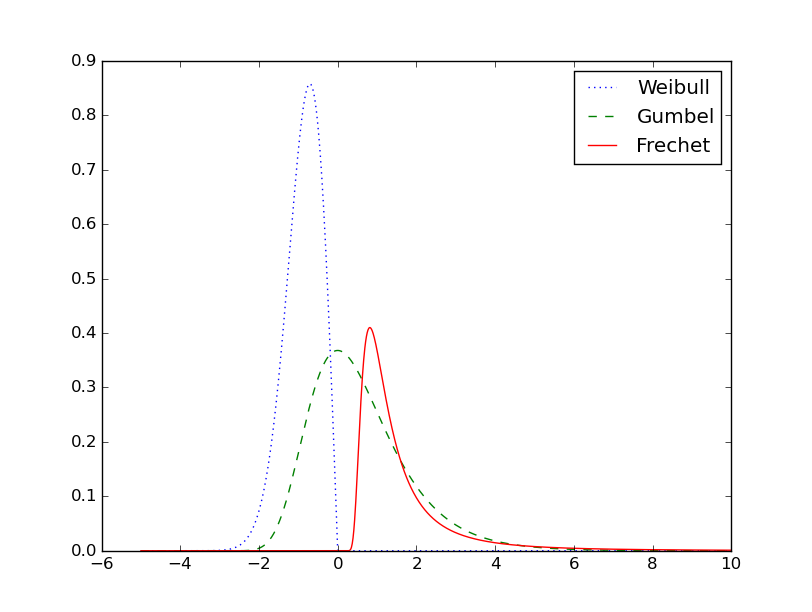
\includegraphics[width=.9\linewidth]{fig_source/GEV.png}
  \caption{Extreme Value Distribution with $\alpha = 2$}
  \label{fig:GEV}
\end{figure}

These extreme value distributions plotted in Figure~\ref{fig:GEV} can be summarized into the so-called Generalized Extreme Value (GEV) Distribution,
% $G(x) = \exp \left(-\left[1 + \gamma \frac{x-\mu}{\sigma}\right]^{-1/\gamma}\right),$
% defined on the set $\{x, 1+ \gamma \frac{x-\mu}{\sigma} > 0\}$ 
% or up to a re-scaling 
\begin{align}
\label{eq:GEV}
G(x) = \exp \left(-\left[1 + \gamma x\right]^{-1/\gamma}\right)
\end{align}
for $1 + \gamma x > 0$, $\gamma \in \mathbb{R}$,
setting by convention $(1 + \gamma x)^{-1/\gamma} = e^{-x}$ for
$\gamma = 0$ (continuous extension). % The sign of $\gamma$ controls the shape of the tail and
% various estimators of the re-scaling sequence and of the shape index $\gamma$ as well have
% been studied in great detail, see \emph{e.g.}  \cite{DEd1989},
% \cite{ELL2009}, 
% \cite{Hill1975}, \cite{Smith1987}, \cite{BVT1996}.
The sign of $\gamma$ controls the shape of the tail of $F$.
 In the case $\gamma >0$ (as for the Cauchy distribution), $G$ is referred to as a Fréchet distribution and $F$ has a heavy tail. If $\gamma=0$ (as for normal distributions), $G$ is a Gumbel distribution and $F$ has a light tail. If $\gamma < 0$ (as for uniform distributions), $G$ is called a Weibull distribution and $F$ has a finite endpoint.
Estimates of univariate extreme quantiles then rely on estimates of the parameters $a_n$, $b_n$, and $\gamma$, see \cite{DEd1989}, \cite{ELL2009}. 
The Hill estimator or one of its generalizations, see \cite{Hill1975}, \cite{Smith1987}, \cite{BVT1996}, provides an estimate of the tail parameter $\gamma$. 
\begin{example}
\begin{itemize}
\item Assume the $X_i$'s to be standard exponential variables (their cdf is $F(x) = 1 - e^{-x}$). In that case, letting $a_n=1$ and $b_n = \log(n)$, we have
$\mathbb{P}[(M_n-b_n)/a_n \le z] = \mathbb{P}[X_1 \le z + \log n ]^n = [1 - e^{-z}/n]^n \to \exp(-e^{-z}) $, for $z \in \rset$. The limit distribution is of Gumbel type ($\xi = 0$).
\item If the $X_i$'s are standard Fréchet ($F(x) = \exp{-1/z}$), letting $an = n$ and $b_n = 0$, one has immediatly $\mathbb{P}[(M_n-b_n)/a_n \le z] = F^n(nz) = \exp(-1/z)$, for $z >0$. The limit distribution remains the Fréchet one ($\xi = 1$).
\item If the $X_i$'s are uniform on $[0,1]$, letting $a_n = 1/n$ and $b_n = 1$, one has $\mathbb{P}[(M_n-b_n)/a_n \le z] = F^n(n^{-1}z + 1) \to \exp(z)$, for $z <0$. The limit distribution is the Weibull one ($\xi = -1$).

\end{itemize}
\end{example}

% Theorem~\ref{thm:univariate-evt} can be reformulated in the following way.
% Suppose there exists two
% sequences $\{a_n, n \ge 1\}$ and $\{b_n, n \ge 1\}$, the $a_n$'s being
% positive, and a non-degenerate distribution function $G$ such that
One can establish an equivalent formulation of Assumption~\eqref{eq:hyp-GEV} which does not rely anymore on the maximum $M_n$:
\begin{align}
\label{eq:hyp-GEV2} %instead of\label{intro:assumption1}
\lim_{n \to \infty} n ~\mathbb{P}\left( \frac{X - b_n}{a_n} ~\ge~ x \right) = -\log G(x)
\end{align}
for all continuity points $x \in \mathbb{R}$ of $G$.
The intuition behind this equivalence is that $$- \log(F^n(a_n x + b_n)) \sim n (1 - F(a_n X + b_n)) = n ~\mathbb{P}\left( \frac{X - b_n}{a_n}~\ge~ x \right)$$ when $n \to \infty$ as $F(a_n X + b_n) \sim 1$.
 The tail behavior of $F$
is then essentially characterized by $G$, which is proved to be -- up
to  re-scaling -- of the type~\eqref{eq:GEV}. 
\medskip
Note that Assumption~\eqref{eq:hyp-GEV} (or \eqref{eq:hyp-GEV2}) is fulfilled for most textbook distributions. In that case $F$ is said to lie in the \textit{domain of  attraction} of $G$, written $F \in DA(G)$.

%XXXXXXXXXXXXXXXXXXXXXXXXXXXXXXXXXXXXXXXXXXXXXXXXXXXXXXXXXXXXXXXXXXXXXXXXXXXXXXXXXXXXXXXXXXXXXXX
% Throughout this paper, for $a_j, b_j \in [0, \infty],~1 \le j \le d$ we use the notations $[a,b]=[a_1,b_1] \times ... \times[a_d,b_d]$ and for $T>0$, $0 \le x \le T$ means $0 \le x_1,...,x_d \le T$.
% Let $\mathbf{X_1,X_2,...,X_n}$ be iid random vectors in $\mathbb{R}^d$ with common distribution function $F$ and marginal distribution functions $F_1,...,F_d$.

\section{Extension to the Multivariate framework}
\label{back:sec:MEVT} 

Extensions to the multivariate setting are well understood
from a probabilistic point of view, but far from obvious from a
statistical perspective. Indeed, the tail dependence structure, ruling the possible simultaneous occurrence of large observations in several directions, has no finite-dimensional parametrization.

The analogue of Assumption (\ref{eq:hyp-GEV2}) for a $d$-dimensional \rv~$\mb X = (X^1,\; \ldots, \; X^d)$ with distribution $\mb F(\mb x):=\mathbb{P}(X_1 \le x_1, \ldots, X_d \le x_d)$, written $\mb F \in \textbf{DA} (\mb G)$ stipulates the existence of two sequences $\{\mb a_n, n \ge 1\}$ and $\{\mb b_n, n \ge 1\}$ in $\mathbb{R}^d$, the $\mb a_n$'s being positive,
and a non-degenerate distribution function $\mb G$ such that
\begin{align}
\label{eq:hyp-GEV2-mult}%\label{intro:assumption2}
\lim_{n \to \infty} n ~\mathbb{P}\left( \frac{X^1 - b_n^1}{a_n^1} ~\ge~ x_1 \text{~or~} \ldots \text{~or~} \frac{X^d - b_n^d}{a_n^d} ~\ge~ x_d \right) = -\log \mb G(\mathbf{x})
\end{align}
% \begin{align}
% \label{intro:assumption2}
% \lim_{n \to \infty} \mathbb{P}\left( \frac{\max_{1 \le i \le n} X_i^1 - b_n^1}{a_n^1} ~\le~ x_1, \ldots, \frac{\max_{1 \le i \le n} X_i^d - b_n^d}{a_n^d} ~\le~ x_d \right) =: G(x)
% \end{align}
for all continuity points $\mathbf{x} \in \mathbb{R}^d$ of $\mb G$. This clearly implies
that the margins $G_1(x_1),\ldots,G_d(x_d)$ are univariate extreme
value distributions, namely of the type $G_j(x) = \exp(-(1 + \gamma_j
x)^{-1/\gamma_j})$. Also, denoting by $F_1,\; \ldots,\; F_d$ the
marginal
distributions of $\mb F$, Assumption~\eqref{eq:hyp-GEV2-mult} implies marginal convergence: $F_i \in DA(G_i)$ for $i=1,\; \ldots,\; n$.
 To understand %capture 
the structure of the limit $\mb G$ and dispose of the
 unknown sequences $(\mb a_n, \mb b_n)$ (which are entirely determined by the
 marginal distributions $F_j$'s), % It is  mathematically very convenient to decompose the joint distribution of $\mb X = (X^1,\ldots, X^d)$ into the margins on the one hand, and the dependence structure on the other hand.
 it is convenient to
 work with marginally standardized variables, that is, to separate the margins from the dependence structure in the description of the joint distribution of $\mb X$. Consider the standardized variables 
 $V^j =1/(1-F_j(X^j))$ and $\mathbf{V}=(V^1,\; \ldots,\; V^d)$.  In
 fact (see Proposition 5.10 in \cite{Resnick1987}), Assumption~\eqref{eq:hyp-GEV2-mult} is
 equivalent to:

\begin{itemize}
\item  marginal convergences $F_j \in DA(G_j)$ as in (\ref{eq:hyp-GEV2}),  % of the marginal distributions \ie~$F_i \in DA(G_i)$, $i=1,\ldots,n$,
 together with 
\item standard  multivariate regular variation of $\mathbf{V}$'s
 distribution,  which means existence of a limit measure $\mu$  on $ [0,\infty]^d\setminus\{\mb 0\}$ such that % convergence of
\begin{align}
\label{back:intro:regvar}
 n~ \mathbb{P}\left( \frac{V^1 }{n} ~\ge~ v_1 \text{~or~} \cdots
   \text{~or~} \frac{V^d }{n} ~\ge~ v_d \right) \xrightarrow[n\to\infty]{}\mu \left([\mb 0,\mb v]^c\right),
\end{align}
where $[\mb 0,\mathbf{v}]:=[0,\; v_1]\times \cdots \times
[0,\; v_d]$.
\end{itemize}

 Thus the variable $\mb V$ satisfies
(\ref{eq:hyp-GEV2-mult}) with $\mb a_n = \mb n = (n,\; \ldots,\; n)$, $\mb b_n =\mb 0 =(0,\; \ldots,\; 0)$. 

\begin{remark} %XXX to be verified
The standardization in $V$ allows to study the same extreme value distribution for each marginal, and with the same re-scaling sequences $a_n$ and $b_n$ for each marginal. In the case of Pareto standardization like here, the underlying extreme value distribution is the Fréchet one.
\end{remark}

The dependence structure of the limit $\mb G$ in (\ref{eq:hyp-GEV2-mult})
can be expressed by means of the so-termed \textit{exponent measure} $\mu$: 
\begin{align}
- \log \mb G(\mathbf{x})= \mu\left( \left[ \mb 0, \left(\frac{-1}{\log G_1(x_1)}, \dots ,\frac{-1}{\log G_d(x_d)}\right)\right]^c\right). \nonumber
\end{align}
The latter  is finite on
sets bounded away from $\mb 0$ and has the
homogeneity property : $\mu(t\point) =
t^{-1}\mu(\point)$. Observe in addition that, due to the standardization chosen (with
`nearly' Pareto margins), the support of $\mu$ is included in $[\mb 0,\; \mathbf{1}]^c$. % then be written using the stable
% tail dependence function ({\sc stdf}) $l$ :
% \begin{align*}
% G(\mathbf{x})=\exp (~ -l(-\log G_1(x_1), \dots ,-\log G_d(x_d)~ )
% \end{align*}
%The so-called \emph{exponent measure} $\mu$ is finite on
%sets bounded away from $0$ and has the
%homogeneity property : $\mu(t\point) =
%t^{-1}\mu(\point)$. Further, due to our standardization choice to
%`nearly' Pareto margins, it can be shown that 
%\begin{align}
 % \label{eq:normalizing_mu_vj_ge1}
 % \mu\{\mb v~:v_j>1\} = 1\;;\qquad j=1\,\ldots,d.
%\end{align}
 To wit, the measure $\mu$ should be viewed, up to a a normalizing factor, as
the asymptotic distribution of $\mb V$ in extreme regions. For any borelian subset $A$ bounded away from $\mb 0$ on which $\mu$ is continuous, we have 
\begin{align}
\label{eq:regularVariation}
t~ \mathbb{P}\left( \mb V \in t A\right) \xrightarrow[t\to\infty]{}\mu(A).     
\end{align}
Using the homogeneity property $\mu(t\point) =
t^{-1}\mu(\point)$, one may show
that $\mu$  can be decomposed into a  radial component and an angular component
$\Phi$, which are independent from each other (see \emph{e.g.} \cite{dR1977}).
Indeed, for all $\mb v = (v_1,...,v_d) \in \mathbb{R}^d$, set
\begin{align}\label{eq:pseudoPolar_change}
  \left\{ \begin{aligned}
R(\mb v)&:= \|\mb v\|_\infty ~=~ \max_{i=1}^d v_i, \\
\Theta (\mb v) &:= \left( \frac{v_1}{R(\mb v)},..., \frac{v_d}{R(\mb v)} \right)
\in S_\infty^{d-1},     
  \end{aligned}\right.
\end{align}
where $S_\infty^{d-1}$ is the positive orthant of  the unit sphere in $\mathbb{R}^d$ for the infinity norm.
Define the \emph{ spectral measure} (also called \emph{angular measure}) by $\Phi(B)= \mu (\{\mb v~:~R(\mb v)>1 ,
\Theta(\mb v) \in B \})$. Then, for every $B
\subset S_\infty^{d-1}$, 
\begin{align}
\label{mu-phi}
\mu\{\mb v~:~R(\mb v)>z, \Theta(\mb v) \in B \} = z^{-1} \Phi (B)~. 
\end{align}
In a nutshell,  there
is a one-to-one correspondence between the exponent measure $\mu$ and the angular measure
$\Phi$, both of them can be used to characterize the asymptotic tail
dependence of the distribution $\mb F$ (as
soon as the  margins $F_j$ are known), since   % after each marginal had been standardized in $\mathbf{U}$ or $\mathbf{V}$.
\begin{align}\label{eq:integratePhiLambda}
  \mu \big( [\mb 0,\mathbf{x}^{-1}]^c \big) =  \int_{\boldsymbol{\theta} \in S_{\infty}^{d-1}}   \max_j{\boldsymbol{\theta}_j x_j} \;\ud \Phi(\boldsymbol{\theta}),
\end{align}
%where $S^{d-1}:= \{w \in [0,1]^d, w_1+\ldots w_d =1\}$, and 
this equality being obtained from the change of variable~\eqref{eq:pseudoPolar_change} , see \emph{e.g.} Proposition 5.11 in \cite{Resnick1987}. 
Recall that here and beyond, operators on vectors are understood component-wise, so that $\mb x^{-1}=(x_1^{-1},\ldots,x_d^{_1})$.
The angular measure can be seen as the asymptotic conditional distribution of the
`angle' $\Theta$ given that the radius $R$ is large, up to the
normalizing constant $\Phi(S_\infty^{d-1})$. Indeed, dropping
the dependence on $\mb V$ for convenience, we have for any
\emph{continuity set} $A$ of $\Phi$, 
\begin{align}
  \label{eq:limitConditAngle}
\begin{aligned}
  \PP(\Theta \in A ~|~R>r ) &= 
\frac{r  \PP(\Theta \in A , R>r ) }{r\PP(R>r)} 
& \xrightarrow[r\to \infty]{} \frac{\Phi(A)}{\Phi(S_\infty^{d-1})} .
\end{aligned}  
\end{align}
The choice of the marginal standardization is somewhat arbitrary and alternative standardizations  lead
to different limits. Another common choice consists in considering `nearly
uniform' 
variables (namely, uniform variables when the margins are continuous): defining $\mathbf{U}$ by $U^j =1-F_j(X^j)$ for
$j\in\{1,\ldots,d\}$,   % the existence of the limit in (\ref{eq:hyp-GEV2-mult}) is then equivalent to each
% of the following conditions (with the notations $\mathbf{x}^{-1}=(x_1^{-1},\ldots,x_d^{-1})$ and $[0,\mathbf{x}]=[0,x_1]\times \ldots \times [0,x_d]$) :
condition (\ref{back:intro:regvar}) is equivalent to each of the  following conditions:
\begin{itemize}
\item $\mathbf{U}$ has  `inverse multivariate regular variation' % on $[0,\infty]^d \setminus \{\infty\}$
  with limit measure $\Lambda(\point)$ $:=\mu((\point)^{-1})$, namely,
  for every measurable set $A$ bounded away from $+\boldsymbol{\infty}$ which is a
  continuity set of $\Lambda$,
\begin{align}
\label{back:reg_var_U}
t~ \mathbb{P}\left( \mb U \in t^{-1} A\right)
\xrightarrow[t\to\infty]{} \Lambda(A) = \mu(A^{-1}), 
\end{align}
where $A^{-1} = \{\mb u \in \rset^{d}_+ ~:~(u_1^{-1},\ldots,u_d^{-1})
\in A\}$. The limit measure $\Lambda$ is finite on sets bounded away from $\{+\boldsymbol{\infty}\}$. 
\item The \textit{stable tail dependence function} (\stdf) defined for $\mb x\in[\mb 0,\boldsymbol{\infty}], \mb x\neq\boldsymbol{\infty}$ by 
\begin{align}
\label{back:stdf1}
l(\mb x) = \lim_{t \to 0} t^{-1} \mathbb{P} \left( U^1 \le t\, x_1 ~\text{or}~ \ldots ~\text{or}~ U^d \le t\,x_d  \right)
 = \mu\left([\mb 0, \mb{x}^{-1}]^c\right) 
\end{align}
exists. 
\end{itemize}

As a conclusion, in multivariate extremes, the focus is on the dependence structure which is characterized by different quantities, such as the exponent measure $\mu$ (itself characterized by its angular part $\Phi$) or the \stdf, which is closely linked to other integrated version of $\mu$ such as extreme-value copula or tail copula. For details on such functionals, see~\cite{Segers12}.
The fact that these quantities characterize the dependence structure can be illustrated by the link they exhibit between the multivariate GEV $G(x)$ and the marginal ones $G_j(x_j),~1 \le j \le d$,

\begin{align*}
- \log \mb G(\mathbf{x})~&=~ \mu\left( \left[ \mb 0, \left(\frac{-1}{\log G_1(x_1)}, \dots ,\frac{-1}{\log G_d(x_d)}\right)\right]^c\right) ~~~~~\text{for the exponent measure,}\\
 - \log \mb G(\mb x) ~&=~ l(-\log G_1(x_1), \ldots, -\log G_d(x_d)) ~~~~~~~~~~~~~~~~~~~~ \text{for the \stdf,}\\
 G( \mb x) ~&=~ C(G_1(x_1), \ldots, G_d(x_d)) ~~~~~~~~~~~~~~~~~~~~~~~~~~~~~~~~~~~~~ \text{for the extreme value copula } C.
\end{align*}


In Chapter~\ref{colt}, we develop non-asymptotic bounds for non-parametric estimation of the \stdf.
As in many applications, it can be more convenient to work with the angular measure itself -- the latter gives more direct information on the dependence structure --, Chapter~\ref{jmva} generalizes the study in Chapter~\ref{colt} to the angular measure.


%XXX commments on these assumptions
% \begin{assumption}\label{hypo:M}
% For every $\beta$ such that $|\beta| > 2$,~ $M_\beta$ is finite and $|\beta_1| \le |\beta_2| \Rightarrow M_{\beta_1} \ge M_{\beta_2}$.
% \end{assumption}
% One 'parcimony assumption' would be something like $M_\beta\le e^{-|\beta|}$.

% In other words we select, for each feature $j\le d$, the `$k$ largest values' $X_i^j$
% over the $n$ observations. According to the nature of the extremal dependence,
% a number between $k$ and $dk$ of observations are selected: $k$ in
% case of perfect dependence, $dk$ in case of `asymptotic independence', which
% means, in EVT, that the components may only be large one at a time. In
% any case, the number of observations considered as extreme is proportionnal to $k$, whence the normalizing factor $\frac{n}{k}$. 

%


% Yet the goal is to study the dependence between the $V_i^j$, $i$ fixed anf $j$ varying.
% One way to proceed is to characterize, for each subset of features
% $\alpha \subset \{1,...,d\}$, the `correlation' of these features
% given that one of them at least  is large and the others are small. %extreme (\ie~given that the observation is extreme).
% Formally, we  associate to each such $\alpha$ a coefficient
% $\mu_n^\alpha$ reflecting the degree of dependence between the
% features $\alpha$. Theoretically, by definition of asymptotic
% dependence, this coeficient is to be proportional to the expected number of
% points $V$ verifying $V^j > 0$, $j \in \alpha$ and $V^j = 0,~ j\notin
% \alpha$, and $\|V\|_\infty\ge r$, namely $ r^{-1}V \in \mathcal{C}_\alpha$ with 
% \begin{align}
% %\label{cone}
% \mathcal{C}_\alpha = \{v \ge 0,~\|v\|_\infty \ge 1,~ v_j > 0 ~\text{ for } j \in \alpha,~ v_j = 0 ~\text{ for } j \notin \alpha \}.
% \end{align}
% (see Fig.~\ref{fig:3Dcones}) But in practice, the data are non-asymptotic so that if $\alpha \neq \{1,\ldots,d\}$ the cones $\mathcal{C}_\alpha$ have zero Lebesgue measure and are not likely to receive empirical mass. Consider then a tolerance parameter $\epsilon>0$ and approximate the asymptotic mass of $~\mathcal{C}_\alpha~$ by the non-asymptotic mass of 
% \begin{align}
%  \label{eq:epsilonCone}
%  ~\mathcal{C}_\alpha^\epsilon~=\{v \ge
%  0,~\|v\|_\infty \ge 1,~ v_j > \epsilon \|v\|_\infty ~\text{ for } j
%  \in \alpha,~v_j \le \epsilon\|v\|_\infty ~\text{ for } j \notin \alpha
%  \} ,
% \end{align}
% which leads to coefficients 

% This motivates the study of the STDF $l$, since it is now theoretically clear how the asymptotic tail dependence structure of $F$ is contained in $l$.
% XXXXXXXXXXXXXXXXXXXXXXXXXXXXXXXXXXXXXXXXXXXXXXXXXXXXXXXXXXXXXXXXXXXXXXXXXXXXXXXXXXXXXXXXXXXXXXXX
% % The measures $\mu$ and $\Lambda$ are called exponent measures and have the following properties:
% % \begin{itemize}
% % \item standardized marginals: for all $a>0$,
% % \begin{align*}
% % \Lambda([0,a]\times[0,\infty]^{d-1})~=~\Lambda([0,\infty]&\times[0,a]\times[0,\infty]^{d-2})
% % \\&~=~...~=~\Lambda([0,\infty]^{d-1}\times[0,a])~=~a
% % \end{align*}
% % \noindent and
% % \begin{align*} 
% % \mu([a,\infty]\times[0,\infty]^{d-1})~=~\mu([0,\infty]&\times[a,\infty]\times[0,\infty]^{d-2})
% % \\&~=~...~=~\mu([0,\infty]^{d-1}\times[a,\infty])~=~a^{-1}
% % \end{align*}
% % \item homogeneity: $\Lambda(c.)=c~ \Lambda(.)$ and $\mu(c.)=c^{-1} \mu(.)$
% % \item concentration: $\Lambda$, $\mu$ are respectively concentrated on $(0,\infty]^d \setminus \{\infty\}$, $[0,\infty)^d \setminus \{0\}$
% % \end{itemize}
% The homogeneity property yields a decomposition of $\mu$ into a
% radial and angular part (see de Haan and Resnick ...). 


\chapter{Background on classical Anomaly Detection algorithms}
\label{back:AD_scikit}
\begin{chapabstract}
  In this chapter, we review some very classical anomaly detection algorithms used in the benchmarks of chapters~\ref{chap:ocrf} and \ref{chap:evaluation}. We also introduce the reader to the scikit-learn library used for illustrative examples. We also present relative implementative contributions of this thesis.%This is also the opportunity to present implementative contributions of this thesis, as two of the algorithms presented here, the Isolation Forest algorithm (Section \ref{sec:iforest}) and the Local Outlier Factor algorithm (Section \ref{sec:lof}), have been implemented on scikit-learn in the context of this Ph.D., as mentioned in the introduction.
\end{chapabstract}

Note: The work on scikit-learn was supervised by Alexandre Gramfort and is the result of a collaboration with the Paris Saclay Center for Data Science. It includes the implementation of Isolation Forest (Section \ref{sec:iforest}) and Local Outlier Factor (Section \ref{sec:lof}) algorithms, as well as a participation to the scikit-learn maintenance and pull requests review.


\section{What is Anomaly Detection?}
Anomaly Detection % (and depending on the application domain, outlier detection, novelty detection, deviation detection, exception mining)
generally consists in assuming that the dataset under study contains a \textit{small} number of anomalies, generated by distribution models that  \textit{differ} from the one generating the vast majority of the data.
 % anomalies are a \textit{small} number of observations generated by \textit{different} models from the one generating the rest of the data
%\sout{ -- the only difference in novelty detection is that the novel patterns are incorporated into the normal model after being detected. }.
This formulation motivates many statistical anomaly detection methods, based on the underlying assumption that anomalies occur in low probability regions of the data generating process. Here and hereafter, the term `normal data' does not refer to Gaussian distributed data, but to \emph{not abnormal} ones, \ie~data belonging to the above mentioned majority. We also call them sometimes \emph{inliers}, while abnormal data are called \emph{outliers}. 
Classical parametric techniques, like those developed by \cite{Barnett94} and \cite{Eskin2000}, assume that the normal data are generated by a distribution belonging to some  specific, known in advance parametric model.  
The most popular non-parametric approaches include algorithms based on density (level set) estimation \citep{Breunig2000LOF, Scholkopf2001, Steinwart2005, Scott2006, VertVert}, on dimensionality reduction \citep{Shyu2003, Aggarwal2001} or on decision trees \citep{Liu2008, Desir12, Shi2012}.
% %approach is statistical, \
% % {\red donner le theme de chaque papier cité}
% \cite{Eskin2000},
% \cite{Desforges1998}, \cite{Barnett94}, \cite{Hawkins1980}
% , distance
% based, \cite{Knorr98}, \cite{Knorr2000}, \cite{Eskin2002geometric},
% local-density based \cite{Breunig2000LOF}, \cite{Breunig99LOF},
% \cite{Tang2002enhancing}, \cite{Papadimitriou2003loci}, spectral based
% \cite{Shyu2003}, \cite{Wang2006}, \cite{Lee2013} and others
% \cite{Aggarwal2001}, \cite{Kriegel2008}, \cite{Liu2008}. 
One may refer to \cite{Hodge2004survey, Chandola2009survey, Patcha2007survey, Markou2003survey} for overviews of current research on Anomaly Detection, ad-hoc techniques being far too numerous to be listed here in an exhaustive manner.


 Most usual anomaly detection algorithms actually
provide more than a predicted label for any new observation, abnormal/normal. Instead,
they return a real valued function,  termed a \textit{scoring function}, defining a preorder/ranking on the input space. Such a function permits to rank any observations according to their supposed `degree of abnormality' and thresholding it yields a decision rule that splits the input space into `normal' and `abnormal' regions.
In various fields (\textit{e.g.} fleet management, monitoring of energy/transportation networks), when confronted with massive data, being able to rank observations according to their degree of abnormality may significantly improve operational processes and allow for a prioritization of actions to be taken, especially in situations where human expertise is required to check each observation is time-consuming.


From a machine learning perspective, anomaly detection can be considered as a specific classification/ranking task, where the usual assumption in supervised learning stipulating that the dataset contains structural information regarding all classes breaks down, see \cite{Roberts99}. This typically happens in the case of two highly unbalanced classes: the normal class is expected to regroup a large majority of the dataset, so that the very small number of points representing the abnormal class does not allow to learn information about this class.
In a clustering based approach, it can be
interpreted as the presence of a single cluster, corresponding to the
normal data. The abnormal ones are too limited to share a commun
structure, \ie~to form a second cluster. Their only characteristic is
precisely to lie outside the normal cluster, namely to lack any
structure.  Thus, common classification approaches may not be applied
as such, even in a supervised
context. % That is the reason why even in a supervised framework, common classification approaches cannot be applied.
\textbf{Supervised} anomaly detection consists in training the algorithm on a labeled (normal/abnormal) dataset including both normal and abnormal observations. In the \textbf{novelty detection} framework (also called \emph{one-class classification} or \emph{semi-supervised} anomaly detection), only normal data are available for training. This is the case in applications where normal operations are known but intrusion/attacks/viruses are unknown and should be detected. In the \textbf{unsupervised} setup (also called \emph{outlier detection}), no assumption is made on the data which consist in unlabeled normal and abnormal instances. In general, a method from the novelty detection framework may apply to the unsupervised one, as soon as the number of anomalies is sufficiently weak to prevent the algorithm from fitting them when learning the normal behavior. Such a method should be robust to outlying observations.

Let us also mention the so-called \emph{semi-supervised novelty detection} \citep{Blanchard2010, Smola2009} framework which is closely linked to the \emph{PU learning framework} \citep{Denis2005, Liu2002, Mordelet2014, duPlessis2015}. 
Semi-supervised novelty detection consists in learning from negative and unsupervised examples, while PU learning consists in learning from positive (P) and unlabeled (U) examples. These hybrid approaches assume that both an unlabeled sample and a sample from one class are available.

In this thesis, we basically place ourselves in the novelty detection framework, although some benchmarks are also done on (unlabeled) training data polluted by outliers, namely in the unsupervised framework.

\section{Three efficient Anomaly Detection Algorithms}
\label{sec:AD_sklearn}


\subsection{One-class SVM}

The SVM algorithm is essentially a two-class algorithm (\ie~one needs negative as well as positive examples).
\cite{Scholkopf2001} extended the SVM methodology to handle training using only positive information:
the One-Class Support Vector Machine (OCSVM) treats the origin as the only member of the second class (after mapping the data to some feature space). Thus the OCSVM finds a separating hyperplane between the origin and the mapped one class. %, using some `relaxation parameters'.

The OCSVM consists in estimating Minimum Volume sets, which amounts (if the density has no flat parts) to estimating density level sets, as mentionned in the introduction.
In \cite{VertVert}, it is shown that the OCSVM is a consistent estimator of density level sets, and that the solution function returned by the OCSVM gives an estimate of the tail of the underlying density.

%
% As a good sketch is better than a long speech, we refer to 
Figures~\ref{table:OCSVM-hard} and \ref{table:OCSVM-soft}  summarizes the theoretical insights of OCSVM compared to the standard SVM, respectively for the hard-margin (no error is tolerated during training) and soft-margin separation (some margin errors are tolerated in training).
\renewcommand{\arraystretch}{2.5}
\begin{table}[!ht]
  \centering
  \begin{tabular}{|c|c|}\hline
    SVM                                                             &    OCSVM  \\ \hline 
    $\displaystyle \min_{w,b} \frac{1}{2} \|w\|^2$                   & $\displaystyle \min_{w} \frac{1}{2} \|w\|^2$   \\
    s.t~~~~ $\forall i,~~y_i(\langle w, x_i\rangle + b) \ge 1$      & s.t~~~~ $\forall i,~~\langle w, x_i\rangle ~\ge 1$ \\ \cdashline{1-2}
    \multicolumn{2}{|l|}{~}\\
    \multicolumn{2}{|l|}{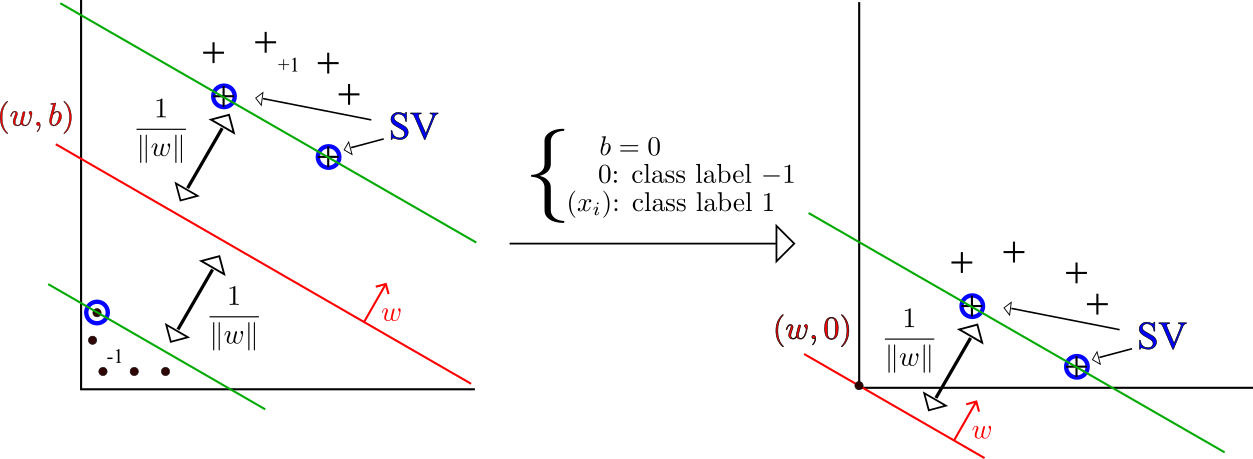
\includegraphics[scale=0.83]{fig_source/OCSVM_hard}} \\\cdashline{1-2}
    decision function:                                             & decision function:  \\
    ~~~~~~~~$f(x) = \text{sgn}(\langle w, x\rangle + b)$ ({\red red line}) ~~~~~~~ & $f(x) = \text{sgn}(\langle w, x\rangle - 1)$ ({\green green line}) \\ \cdashline{1-2} 
    \multicolumn{2}{|l|}{-Lagrange multipliers: $\alpha_i$ ~~~~($\alpha_i>0$ when the constraint is an equality for $x_i$)} \\
    \multicolumn{2}{|l|}{-Support vectors: $\text{SV} = \{ x_i,~~ \alpha_i > 0\}$ }\\
    \multicolumn{2}{|l|}{-Margin errors: $\text{ME} = \emptyset $ ~~~~~~~~~~~~~~~ }\\ \cdashline{1-2}
    $\displaystyle w = \sum_i \alpha_i y_i x_i$                    & $\displaystyle w = \sum_i \alpha_i x_i$  \\ \hline 
  \end{tabular}
  \caption{SVM vs. OCSVM (hard-margin separation)}
  \label{table:OCSVM-hard}
\end{table}

\begin{table}[!ht]
  \centering
  \begin{tabular}{|c|c|}\hline
    SVM                                                             &    OCSVM  \\ \hline 
    $\displaystyle \min_{w,\xi,\rho,b} \frac{1}{2} \|w\|^2 + \frac{1}{n} \sum_{i=1}^n \xi_i - \nu \rho$ & $\displaystyle \min_{w,\xi,\rho} \frac{1}{2} \|w\|^2 + \frac{1}{n} \sum_{i=1}^n \xi_i - \nu \rho$  \\
    s.t~~~~ $\forall i, ~~y_i(\langle w, x_i\rangle ~+~ b) \ge \rho - \xi_i$                        & s.t~~~~ $\forall i,~~\langle w, x_i\rangle ~\ge \rho - \xi_i $ ~~~~~~\\ 
    $\xi_i \ge 0$ ~~~~~~~~~~~~~~~~~~~~~                                                            & $\xi_i \ge 0$~~~~~~~~~~~~  \\ \cdashline{1-2}
    \multicolumn{2}{|l|}{~}\\
    \multicolumn{2}{|l|}{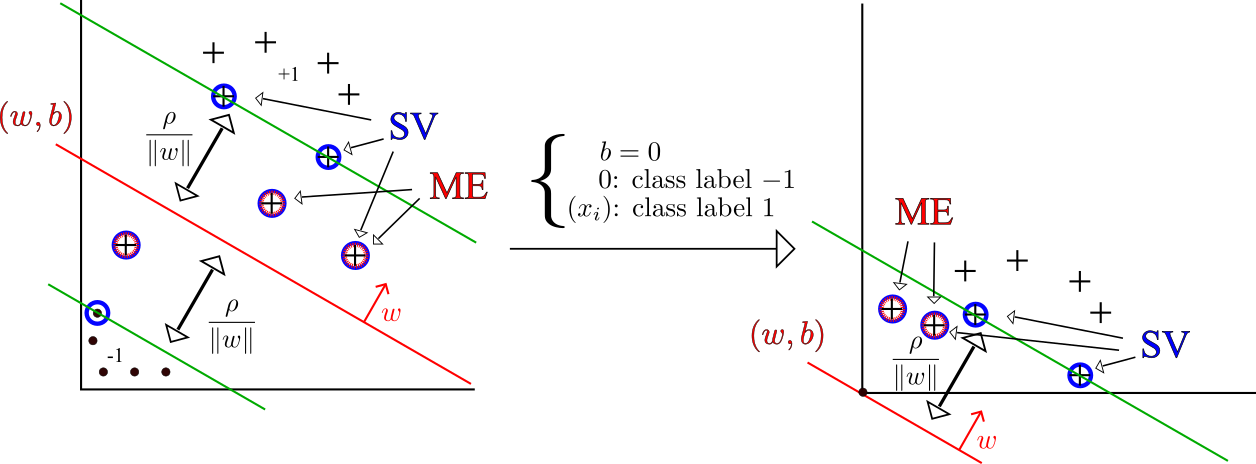
\includegraphics[scale=0.83]{fig_source/OCSVM_soft}} \\\cdashline{1-2}
    decision function:                                                                             & decision function:  \\
    ~~~~~~~~$f(x) = \text{sgn}(\langle w, x\rangle + b)$ ({\red red line}) ~~~~~~~            & $f(x) = \text{sgn}(\langle w, x\rangle - \rho)$ ({\green green line})\\ \cdashline{1-2}
    \multicolumn{2}{|l|}{-Lagrange multipliers: $\alpha_i, \beta_i$ ~~~~(one for each constraint, $\beta_i > 0$ when $\xi_i = 0$)}\\
    \multicolumn{2}{|l|}{-Support vectors: $\text{SV} = \{ x_i,~~ \alpha_i > 0\}$ }\\
    \multicolumn{2}{|l|}{-Margin errors: $\text{ME} = \{x_i,~~ \xi_i > 0 \} =  \{x_i,~~ \beta_i > 0 \} $ ~~~(for OCSVM, ME=anomalies) }\\
    \multicolumn{2}{|l|}{-$\text{SV} \setminus \text{ME} = \{ x_i,~~ \alpha_i, \beta_i > 0\}$ }\\ \cdashline{1-2}
    $w = \sum_i \alpha_i y_i x_i$                                                                   & $w = \sum_i \alpha_i x_i$  \\ \cdashline{1-2}
    \multicolumn{2}{|c|}{ $\displaystyle \frac{|\text{ME}|}{n} ~\le~ \nu ~\le~ \frac{|\text{SV}|}{n}$ }   \\
    \multicolumn{2}{|c|}{$\displaystyle \rho = \langle w, x_i\rangle ~~~~\forall x_i \in \text{SV} \setminus \text{ME}$} \\ \hline

              
  \end{tabular}
  \caption{SVM vs. OCSVM ($\nu$-soft margin separation)}
  \label{table:OCSVM-soft}
\end{table}

In the $\nu$-soft margin separation framework, letting $\Phi$ be the mapping function determined by a kernel function $k$ (\ie~$k(x,y) = \langle \Phi(x), \Phi(y)\rangle$), the separating hyperplane defined \wrt~a vector $w$ and an offset $\rho$ is given by the solution of 
\begin{align*}
&\min_{w,\xi,\rho} \frac{1}{2} \|w\|^2 + \frac{1}{n} \sum_{i=1}^n \xi_i - \nu \rho\\
&\text{s.t.}~~~ \langle w, \Phi(x_i)\rangle ~\ge \rho - \xi_i~~,~~~~~~1 \le i \le n \\
& ~~~~~~~~\xi_i \ge 0,
\end{align*}
where $\nu$ is previously set. An interesting fact is that $\nu$ is an upper bound on the fraction of outliers and a lower bound on the fraction of support vectors, both of which converging to $\nu$ almost surely as $n \to \infty$ (under some continuity assumption). Then, the empirical mass of the estimated level set is greater than $1-\nu$ and converges almost surely to $1-\nu$ as $n$ tends to infinity. Hence one usual approach is to choose $\nu = 1 - \alpha$ to estimate a MV-set with mass (at least) $\alpha$. For insights on the calibration of One-Class SVM, see for instance \cite{Thomas2015}.
%
The OCSVM is mainly applied with Gaussian kernels and its performance highly depends on the kernel bandwidth selection.
The complexity of OCSVM training is the same as for the standard SVM, namely $O(n^3 d)$ where $n$ is the number of samples and $d$ the dimension of the input space. However, one can often expect a complexity of $O(n^2 d)$, see \cite{Bottou2007}. From its linear complexity \wrt~the number of features $d$, OCSVM scales well in large dimension, and performance remains good even when the dimension is greater than $n$. By using only a small subset of the training dataset (support vectors) in the decision function, it is memory efficient. However, OCSVM suffers from practical limitation: 1) the non-linear training complexity in the number of observations, which limits its use on very large datasets; 2) its sensitivity to the parameter $\nu$ and to the kernel bandwidth, which makes calibration tricky; 3) parametrization of the mass of the MV set estimated by the OCSVM via the parameter $\nu$ does not allow to obtain nested set estimates as the mass $\alpha$ increases.

\subsection{Local Outlier Factor algorithm}
\label{sec:lof}
One other very efficient way of performing outlier detection in datasets whose dimension is moderately large is to use the Local Outlier Factor (LOF) algorithm proposed in \cite{Breunig2000LOF}.

This algorithm computes a score reflecting the degree of abnormality of the observations, the so-called local outlier factor. It measures the local deviation of a given data point with respect to its neighbors. By comparing the local density near a sample to the local densities of its neighbors, one can identify points which have a substantially lower density than their neighbors. These are considered to be outliers.

In practice the local density is obtained from the $k$-nearest neighbors. The LOF score of an observation is equal to the ratio of the average local density of his $k$-nearest neighbors, and his own local density: a normal instance is expected to have a local density similar to that of its neighbors, while abnormal data are expected to have much smaller local density.

The strength of the LOF algorithm is that it takes both local and global properties of datasets into consideration: it can perform well even in datasets where abnormal samples have different underlying densities. The question is not, how isolated the sample is, but how isolated it is with respect to the surrounding neighborhood.


\subsection{Isolation Forest}
\label{sec:iforest}


One efficient way of performing outlier detection in high-dimensional datasets
is to use random forests.
%
The IsolationForest proposed in \cite{Liu2008} 'isolates' observations by randomly selecting a feature and then randomly selecting a split value between the maximum and minimum values of the selected feature.
%
Since recursive partitioning can be represented by a tree structure, the
number of splittings required to isolate a sample is equivalent to the path
length from the root node to the terminating node.
%
This path length, averaged over a forest of such random trees, is a measure
of abnormality. The scoring function is based on this averaged depth.
%
Random partitioning produces noticeable shorter paths for anomalies, see figures~\ref{fig:ideeIF} and \ref{fig:convergenceIF}. Moreover, the average depth of a sample over the forest seems to converge to some limits, the latter being different whether the sample is or not an anomaly.
Hence, when a forest of random trees collectively produces shorter path lengths
for particular samples, they are highly likely to be anomalies.
%




\section{Examples through scikit-learn}
\label{back:sklearn-contribution}
This section provides examples on the anomaly detection algorithms presented above through the scikit-learn python library.

As mentioned in the introduction, contribution of this thesis includes the implemention of two classical anomaly detection algorithms on the open-source scikit-learn library (\cite{sklearn2011}), namely the Isolation Forest algorithm (\cite{Liu2008}) and the Local Outlier Factor algorithm (\cite{Breunig2000LOF}). % , which are respectively presented in sections \ref{sec:lof} and \ref{sec:iforest}.
This work was supervised by Alexandre Gramfort and is the result of a collaboration with the Paris Saclay Center for Data Science. It also includes participation to the scikit-learn maintenance and pull requests review.

% by describing and comparing anomaly detection algorithms from this library. Part of this section are modified versions of the documentation included in the forementioned scikit-learn contribution.


\subsection{What is scikit-learn?}
Scikit-learn, see \cite{sklearn2011}, is an open-source library which provides well-established machine learning methods.
It is a Python module, the latter language being very popular for scientific computing, thanks to its high-level interactive nature. Python is enjoying this recent years a strong expansion both in academic and industrial settings. Scikit-learn takes advantage of this favourable backdrop and extends this general-purpose programming language with machine learning operation: It not only provides implementations of many established algorithms, both supervised and unsupervised, while keeping an easy-to-use interface tightly integrated with the Python language. But it also provides a composition mechanism (through a \emph{Pipeline} object) to combine estimators, preprocessing tools and model selection methods in such a way that the user can easily construct complex ad-hoc algorithms.

Scikit-learn depends only on \emph{numpy} (the base data structure used for data and model parameters, see \cite{Vanderwalt2011numpy}) and \emph{scipy} (to handle common numerical operations, see \cite{Jones2015scipy}).
Most of the Scikit-learn package is written in python and \emph{cython}, a compiled programming language for combining C in Python to achieve the performance of C with high-level programming in Python-like syntax.


The development is done on \emph{github}\footnote{https://github.com/scikit-learn}, a Git repository hosting service which facilitates collaboration, as coding is done in strong interaction with other developpers. Because of the large number them, emphasis is put on keeping the project maintainable, \eg~by avoiding dupplicating code.% up to pay (reasonably) in computational performance. As an example, the initial Isolation Forest implementation contained a complementary cython code to efficiently browse the trees of the forest. This functionality was included in an other (more complete) tree browser, but which is heavier in terms of computation. A balance had to be made between the computational gain and the maintainability cost, which led to choose the last one.


Scikit-learn benefits from a simple and consistent API (Application Programming Interface), see \cite{sklearn_api2013}, through the \emph{estimator} interface. This interface is followed by all (supervised and unsupervised) learning algorithms as well as other tasks such as preprocessing, feature extraction and selection. The central object \emph{estimator} implements a \emph{fit} method to learn from training data, taking as argument an input data array (and optionnally an array of labels for supervised problems). The initialization of the estimator is done separately, before training, in such a way the constructor doesn't see any data and can be seen as a function taking as input the model hyper-parameters and returning the learning algorithm initialized with these parameters. Relevant default parameters are provided for each algorithm. To illustrate initialization and fit steps, the snippet below considers an anomaly detection learning task with the \emph{Isolation Forest} algorithm.

\begin{pythoncode} 
# Import the IsolationForest algorithm from the ensemble module
from sklearn.ensemble import IsolationForest

# Instantiate with specified hyper-parameters
IF = IsolationForest(n_trees=100, max_samples=256)

# Fit the model on training data (build the trees of the forest)
IF.fit(X_train)
\end{pythoncode}


In this code example, the Isolation Forest algorithm is imported from the \emph{ensemble} module of scikit-learn, which contains the ensemble-based estimators such as bagging or boosting methods. Then, an $IsolationForest$ instance $IF$ is initialized with a number of trees of $100$ (see Section~\ref{sec:iforest} for details on this algorithm). Finally, the model is learned from training data $X\_train$ and stored on the $IF$ object for later use. Since all estimators share the same API, it is possible to train a Local Outlier Factor algorithm by simply replacing the constructor name $IsolationForest(n\_trees=100)$ in the snippet above by $LocalOutlierFactor()$.

Some estimators (such as supervised estimators or some of the unsupervised ones, like Isolation Forest and LOF algorithm) are called \emph{predictors} and implement a \emph{predict} method that takes a data array and returns predictions (labels or values computed by the model). Other estimators (\eg~PCA) are called \emph{transformer} and implement a \emph{transform} method returning modified input data.
The following code example illustrates how simple it is to predict labels with the predictor interface. It suffices to add the line of code below to the previous snippet.

\begin{pythoncode} 
# Perform prediction on new data
y_pred = IF.predict(X_test)  
# Here y_pred is a vector of binary labels (+1 if inlier, -1 if abnormal)
\end{pythoncode}



\subsection{LOF examples}
The use of LOF algorithm is illustrated in the code example below, returning Figure~\ref{fig:lof}.
\begin{figure}[!ht]
  %\centering
  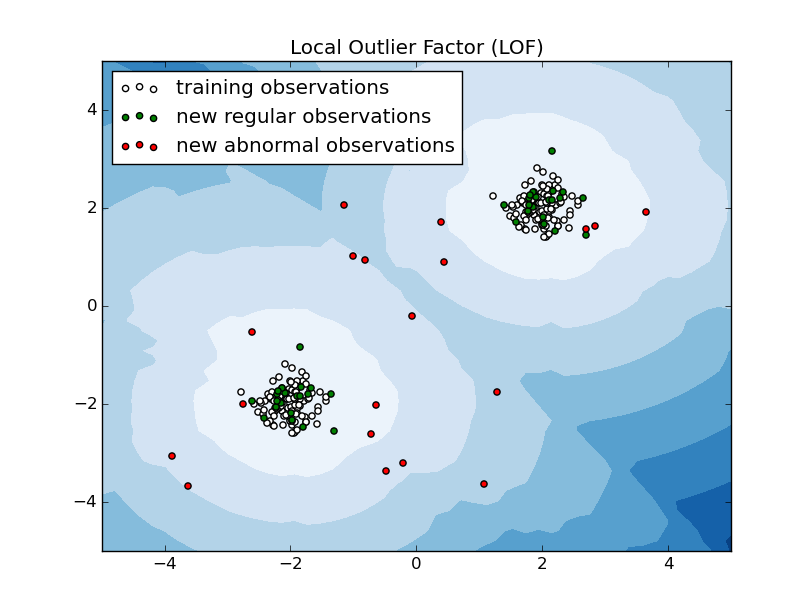
\includegraphics[width=0.9\linewidth]{fig_source/lof}
  \caption{LOF example}
  \label{fig:lof}
\end{figure}

%\begin{pythoncode} 
\begin{mdframed}[hidealllines=true, backgroundcolor=lightgray] 
\begin{minted}[fontfamily=courier, fontsize=\scriptsize]{python}
"""
=================================================
Anomaly detection with Local Outlier Factor (LOF)
=================================================

This example uses the LocalOutlierFactor estimator
for anomaly detection.
"""

import numpy as np
import matplotlib.pyplot as plt
from sklearn.neighbors import LocalOutlierFactor

np.random.seed(42)

# Generate train data
X = 0.3 * np.random.randn(100, 2)
X_train = np.r_[X + 2, X - 2]
# Generate some regular novel observations
X = 0.3 * np.random.randn(20, 2)
X_test = np.r_[X + 2, X - 2]
# Generate some abnormal novel observations
X_outliers = np.random.uniform(low=-4, high=4, size=(20, 2))

# fit the model
clf = LocalOutlierFactor()
clf.fit(X_train)
y_pred_train = clf.predict(X_train)
y_pred_test = clf.predict(X_test)
y_pred_outliers = clf.predict(X_outliers)

# plot the line, the samples, and the nearest vectors to the plane
xx, yy = np.meshgrid(np.linspace(-5, 5, 50), np.linspace(-5, 5, 50))
Z = clf.decision_function(np.c_[xx.ravel(), yy.ravel()])
Z = Z.reshape(xx.shape)

plt.title("Local Outlier Factor (LOF)")
plt.contourf(xx, yy, Z, cmap=plt.cm.Blues_r)

b1 = plt.scatter(X_train[:, 0], X_train[:, 1], c='white')
b2 = plt.scatter(X_test[:, 0], X_test[:, 1], c='green')
c = plt.scatter(X_outliers[:, 0], X_outliers[:, 1], c='red')
plt.axis('tight')
plt.xlim((-5, 5))
plt.ylim((-5, 5))
plt.legend([b1, b2, c],
           ["training observations",
            "new regular observations", "new abnormal observations"],
           loc="upper left")
plt.show()
\end{minted}
\end{mdframed}
%\end{pythoncode}


\subsection{Isolation Forest examples}
The Isolation Forest strategy is illustrated in the code example below returning Figure~\ref{fig:iforest}.


\begin{minipage}{0.52\linewidth}
\centering
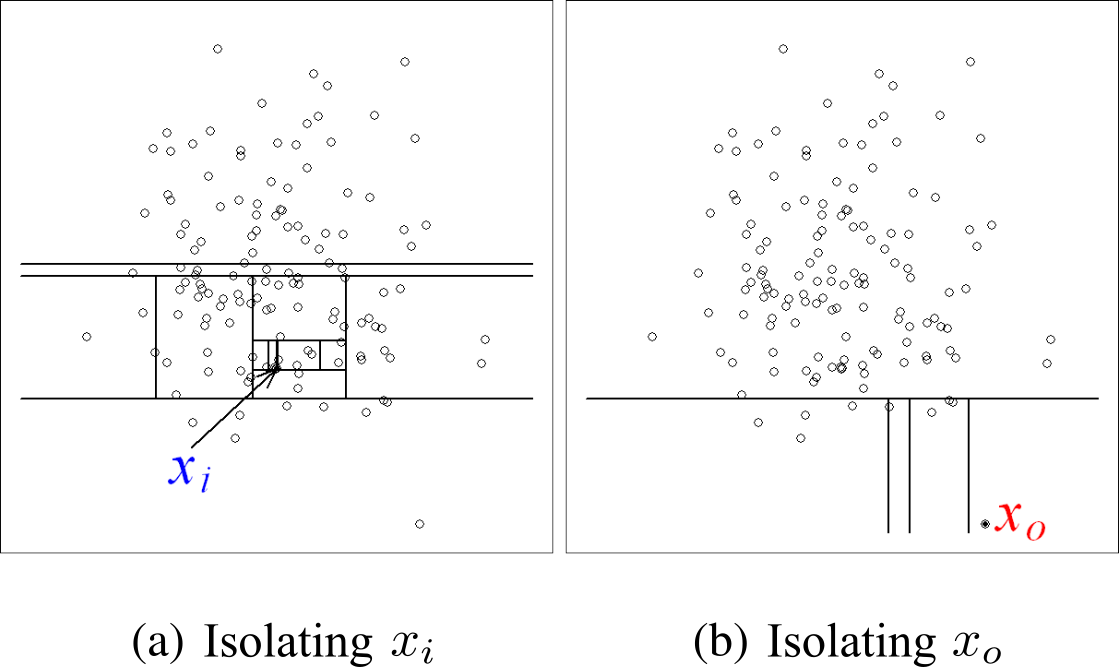
\includegraphics[scale=.95]{fig_source/ideeIF}
\captionof{figure}{Anomalies are isolated more quickly}
\label{fig:ideeIF}
\end{minipage}\hfill
\begin{minipage}{0.52\linewidth}
\centering
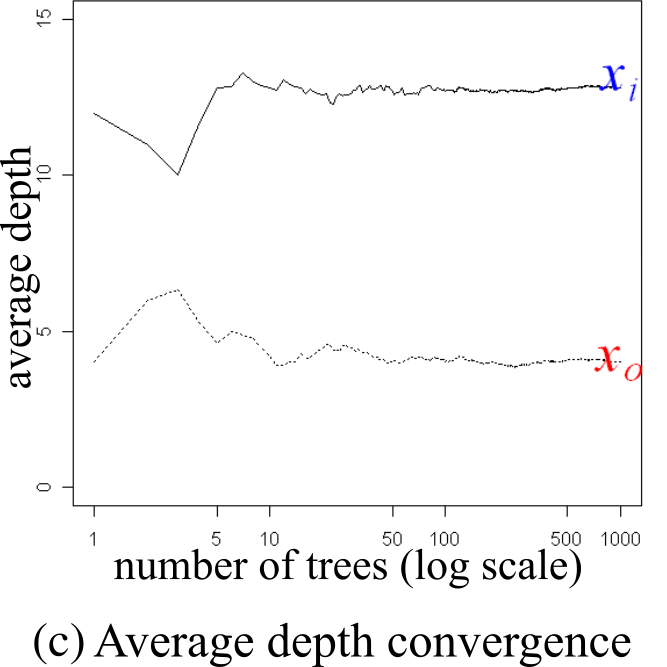
\includegraphics[scale=.95]{fig_source/convergenceIF}
\captionof{figure}{Convergence of the averaged depth}
\label{fig:convergenceIF}
\end{minipage}


\begin{figure}[!ht]
\centering
  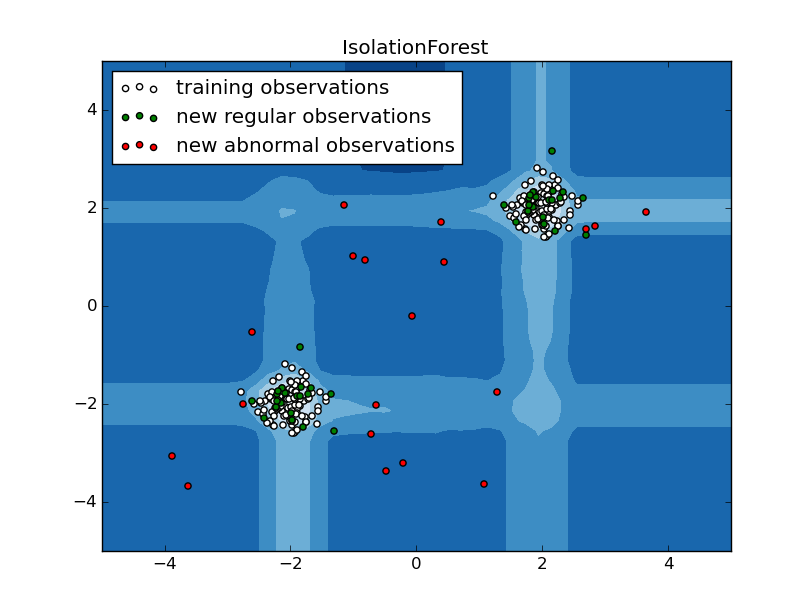
\includegraphics[width=0.8\linewidth]{fig_source/iforest}
  \caption{Isolation Forest example}
  \label{fig:iforest}
\end{figure}
~\\
%\begin{pythoncode} 
\begin{mdframed}[hidealllines=true, backgroundcolor=lightgray] 
\begin{minted}[fontfamily=courier, fontsize=\scriptsize]{python}
"""
==========================================
IsolationForest example
==========================================

An example using IsolationForest for anomaly detection.

"""

import numpy as np
import matplotlib.pyplot as plt
from sklearn.ensemble import IsolationForest

rng = np.random.RandomState(42)

# Generate train data
X = 0.3 * rng.randn(100, 2)
X_train = np.r_[X + 2, X - 2]
# Generate some regular novel observations
X = 0.3 * rng.randn(20, 2)
X_test = np.r_[X + 2, X - 2]
# Generate some abnormal novel observations
X_outliers = rng.uniform(low=-4, high=4, size=(20, 2))

# fit the model
clf = IsolationForest(max_samples=100, random_state=rng)
clf.fit(X_train)
y_pred_train = clf.predict(X_train)
y_pred_test = clf.predict(X_test)
y_pred_outliers = clf.predict(X_outliers)

# plot the line, the samples, and the nearest vectors to the plane
xx, yy = np.meshgrid(np.linspace(-5, 5, 50), np.linspace(-5, 5, 50))
Z = clf.decision_function(np.c_[xx.ravel(), yy.ravel()])
Z = Z.reshape(xx.shape)

plt.title("IsolationForest")
plt.contourf(xx, yy, Z, cmap=plt.cm.Blues_r)

b1 = plt.scatter(X_train[:, 0], X_train[:, 1], c='white')
b2 = plt.scatter(X_test[:, 0], X_test[:, 1], c='green')
c = plt.scatter(X_outliers[:, 0], X_outliers[:, 1], c='red')
plt.axis('tight')
plt.xlim((-5, 5))
plt.ylim((-5, 5))
plt.legend([b1, b2, c],
           ["training observations",
            "new regular observations", "new abnormal observations"],
           loc="upper left")
plt.show()
\end{minted}
\end{mdframed}
%\end{pythoncode}

\subsection{Comparison examples}

As a conclusion,
Figures~\ref{fig:ADcomparison1}, \ref{fig:ADcomparison2} and \ref{fig:ADcomparison3} draw a comparison of the three anomaly detection algorithms introduced in this section:

- the One-Class SVM is able to capture the shape of the
  data set, hence performing well when the data is strongly
  non-Gaussian, i.e. with two well-separated clusters;

- the Isolation Forest algorithm, is adapted to
  large-dimensional settings, even if it performs quite well in the
  examples below.

- the Local Outlier Factor measures the local deviation of a given
  data point with respect to its neighbors by comparing their local density.

The ground truth about inliers and outliers is given by the points colors
while the orange-filled area indicates which points are reported as inliers
by each method.

Here, we assume that we know the fraction of outliers in the datasets.
Thus rather than using the `predict' method of the objects, we set the
threshold on the decision function to separate out the corresponding
fraction. Anomalies are uniformly drawn according to an uniform distribution.


\begin{figure}[H]
  \centering
  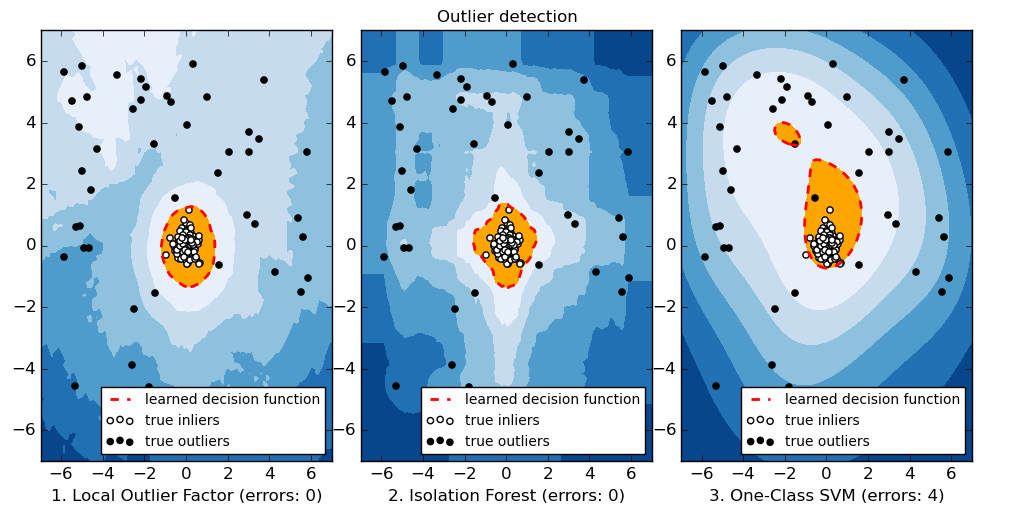
\includegraphics[width=.9\linewidth]{fig_source/ADcomparison1}
  \caption{gaussian normal data with one single mode}
  \label{fig:ADcomparison1}
\end{figure}

\begin{figure}[H]
  \centering
  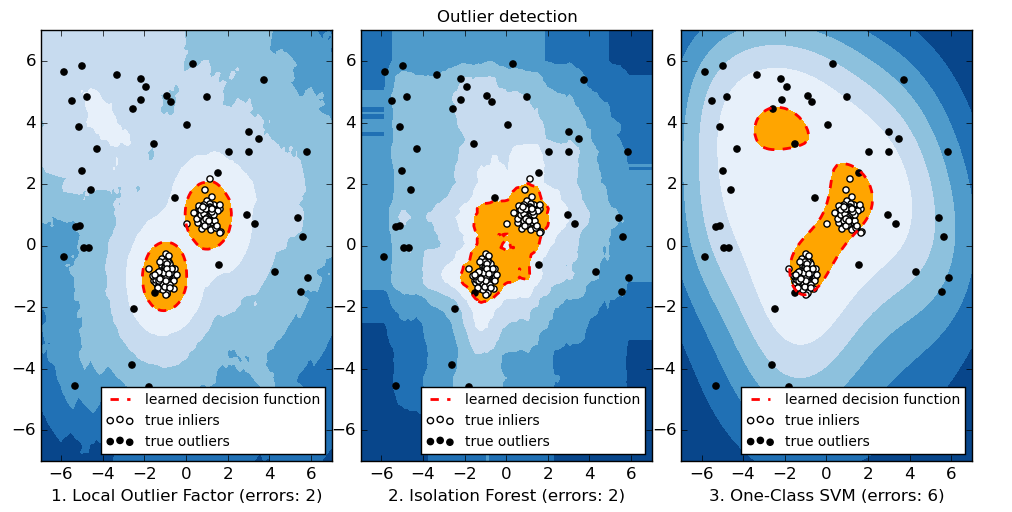
\includegraphics[width=.9\linewidth]{fig_source/ADcomparison2}
  \caption{gaussian normal data with two modes}
  \label{fig:ADcomparison2}
\end{figure}

\begin{figure}[H]
  \centering
  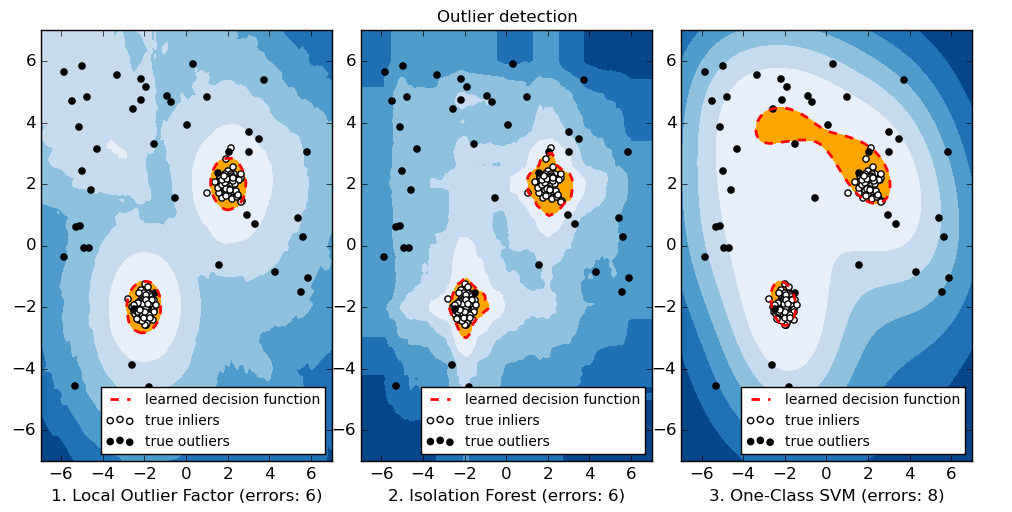
\includegraphics[width=.9\linewidth]{fig_source/ADcomparison3}
  \caption{gaussian normal data with two strongly separate modes}
  \label{fig:ADcomparison3}
\end{figure}

% as the following code is longer than 1 page, bgcolor=lightgray option does not work: we have to use mdframed package
\begin{mdframed}[hidealllines=true, backgroundcolor=lightgray] 
\begin{minted}[fontfamily=courier, fontsize=\scriptsize]{python}
"""
==========================================
Outlier detection with several methods.
==========================================
"""

import numpy as np
import matplotlib.pyplot as plt
import matplotlib.font_manager
from scipy import stats

from sklearn import svm
from sklearn.covariance import EllipticEnvelope
from sklearn.ensemble import IsolationForest
from sklearn.neighbors import LocalOutlierFactor

rng = np.random.RandomState(42)

# Example settings
n_samples = 200
outliers_fraction = 0.25
clusters_separation = [0, 1, 2]

# define two outlier detection tools to be compared
classifiers = {
    "One-Class SVM": svm.OneClassSVM(nu=0.95 * outliers_fraction + 0.05,
                                     kernel="rbf", gamma=0.1),
    #"robust covariance estimator": EllipticEnvelope(contamination=.25),
    "Isolation Forest": IsolationForest(random_state=rng),
    "Local Outlier Factor": LocalOutlierFactor(n_neighbors=35, contamination=0.25)}

# Compare given classifiers under given settings
xx, yy = np.meshgrid(np.linspace(-7, 7, 100), np.linspace(-7, 7, 100))
n_inliers = int((1. - outliers_fraction) * n_samples)
n_outliers = int(outliers_fraction * n_samples)
ground_truth = np.ones(n_samples, dtype=int)
ground_truth[-n_outliers:] = 0

# Fit the problem with varying cluster separation
for i, offset in enumerate(clusters_separation):
    np.random.seed(42)
    # Data generation
    X1 = 0.3 * np.random.randn(n_inliers // 2, 2) - offset
    X2 = 0.3 * np.random.randn(n_inliers // 2, 2) + offset
    X = np.r_[X1, X2]
    # Add outliers
    X = np.r_[X, np.random.uniform(low=-6, high=6, size=(n_outliers, 2))]

    # Fit the model
    plt.figure(figsize=(10, 5))
    for i, (clf_name, clf) in enumerate(classifiers.items()):
        # fit the data and tag outliers
        clf.fit(X)
        y_pred = clf.decision_function(X).ravel()
        threshold = stats.scoreatpercentile(y_pred,
                                            100 * outliers_fraction)
        y_pred = y_pred > threshold
        n_errors = (y_pred != ground_truth).sum()
        # plot the levels lines and the points
        Z = clf.decision_function(np.c_[xx.ravel(), yy.ravel()])
        Z = Z.reshape(xx.shape)
        subplot = plt.subplot(1, 3, i + 1)
        subplot.contourf(xx, yy, Z, levels=np.linspace(Z.min(), threshold, 7),
                         cmap=plt.cm.Blues_r)
        a = subplot.contour(xx, yy, Z, levels=[threshold],
                            linewidths=2, colors='red')
        subplot.contourf(xx, yy, Z, levels=[threshold, Z.max()],
                         colors='orange')
        b = subplot.scatter(X[:-n_outliers, 0], X[:-n_outliers, 1], c='white')
        c = subplot.scatter(X[-n_outliers:, 0], X[-n_outliers:, 1], c='black')
        subplot.axis('tight')
        subplot.legend(
            [a.collections[0], b, c],
            ['learned decision function', 'true inliers', 'true outliers'],
            prop=matplotlib.font_manager.FontProperties(size=10),
            loc='lower right')
        subplot.set_xlabel("%d. %s (errors: %d)" % (i + 1, clf_name, n_errors))
        subplot.set_xlim((-7, 7))
        subplot.set_ylim((-7, 7))
    plt.subplots_adjust(0.04, 0.1, 0.96, 0.94, 0.1, 0.26)
    plt.suptitle("Outlier detection")

plt.show()
\end{minted}
\end{mdframed}


%\chapter{A performance criterion: the Mass-Volume Curve}

%\subsection{Elliptic Envelop}
